%% Beispiel-Präsentation
\documentclass{sdqbeamer}
 
%% Titelbild
\titleimage{banner_2020_kit}

%% Gruppenlogo
\grouplogo{hci}

%% Gruppenname und Breite (Standard: 50 mm)
\groupname{Mensch-Maschine-Interaktion und Barrierefreiheit}
%\groupnamewidth{50mm}

% Beginn der Präsentation

\title[Solidarische Raumnutzung Entwurfsheft]{Kolloquium Entwurfsheft zur Solidarischen Raumnutzung}
\author[Soli-Gruppe]{Alexander Klee, Jannik Hönlinger, Johannes Frohnmeyer, Ben Steinle und Antonia Ammon }
\subtitle{PSE-Projekt WS24/25}
\date[03.\,01.\,2025]{03. Januar 2025}

% Literatur
 
\usepackage[citestyle=authoryear,bibstyle=numeric,hyperref,backend=biber]{biblatex}
\addbibresource{presentation.bib}
\bibhang1em

\begin{document}
 
%Titelseite
\KITtitleframe

%Gliederung
\begin{frame}{Gliederung}
\tableofcontents
\end{frame}

\section{Aufbau}

\subsection{Architektur}

\begin{frame}{Architektur}
\begin{figure}
    \centering
    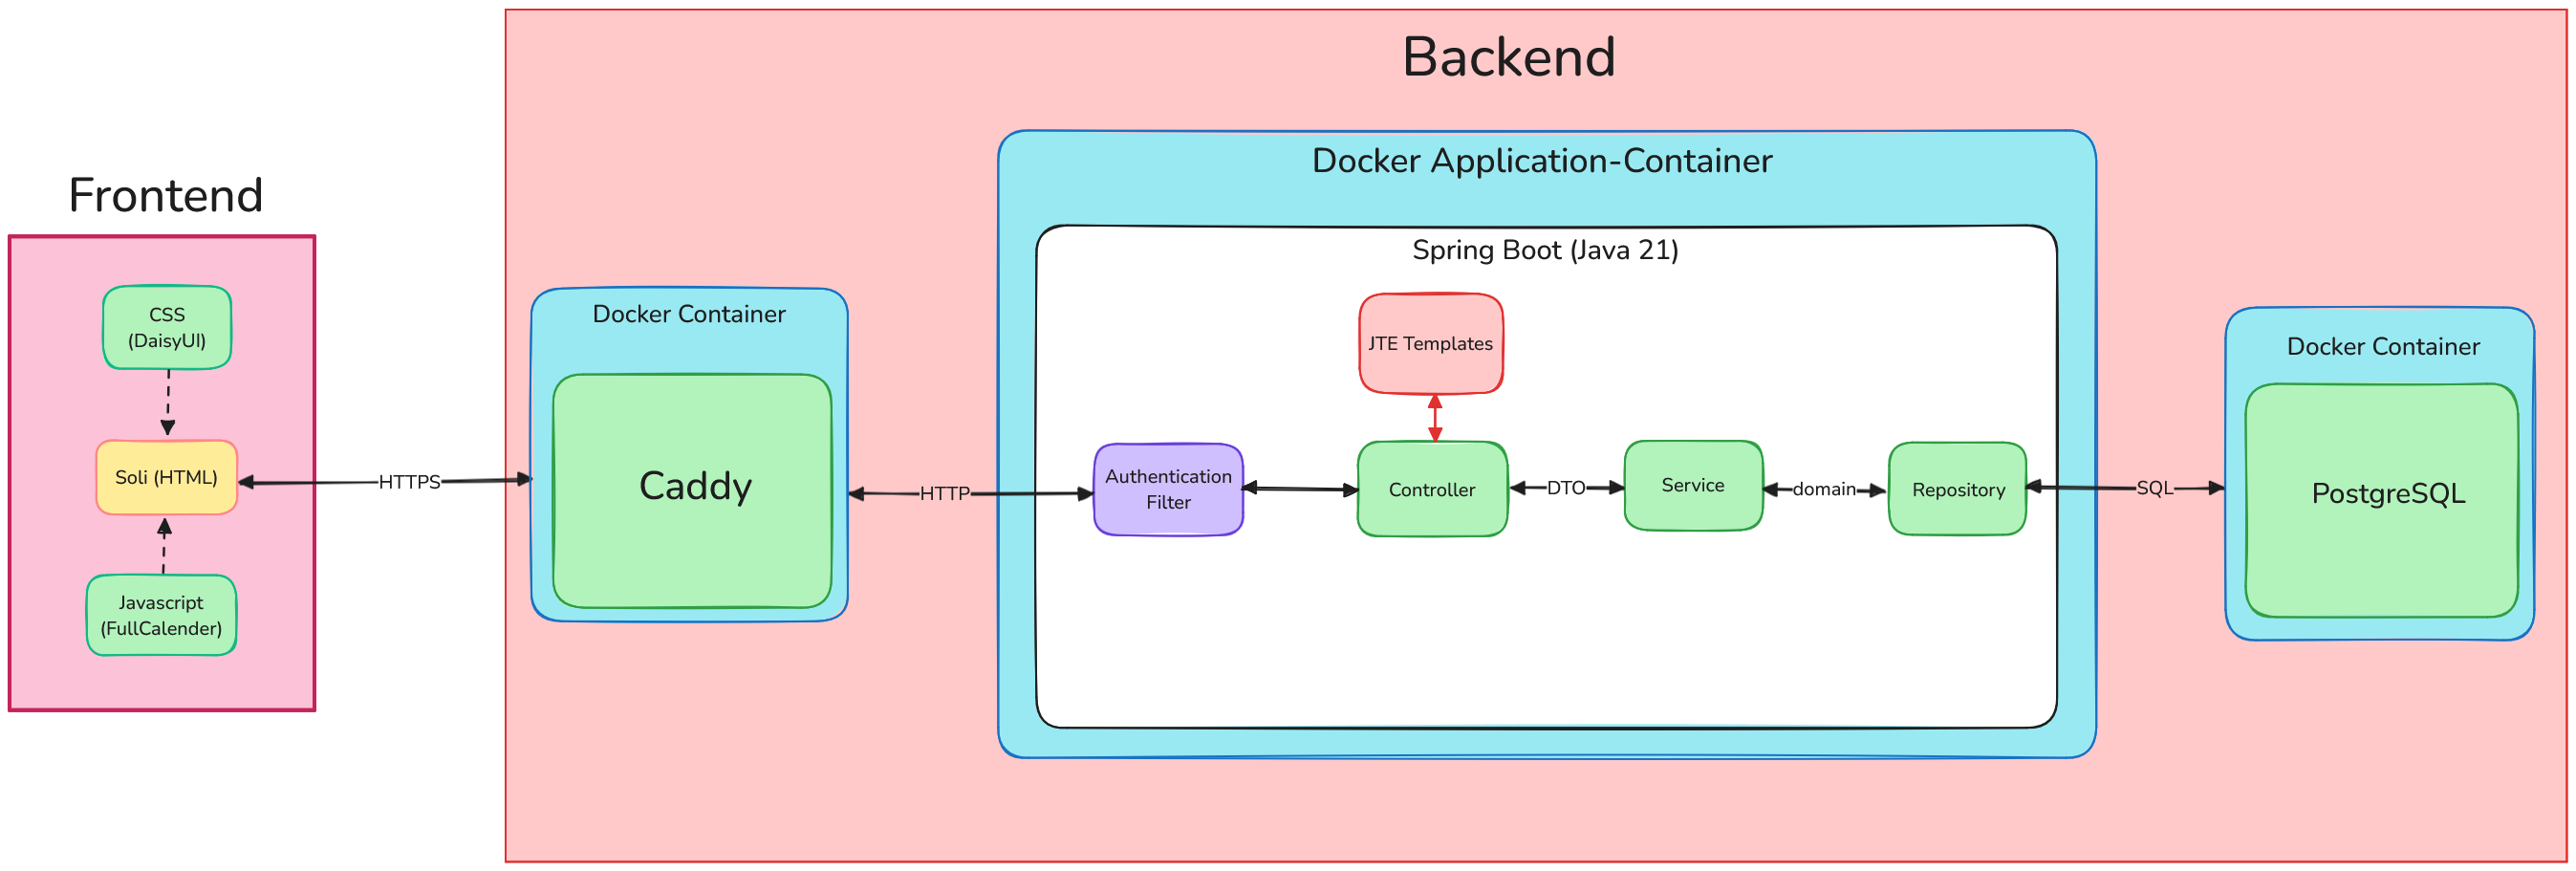
\includegraphics[width=\textwidth]{pictures/figures/architecture}
    \label{fig:architektur}
\end{figure}
\end{frame}

\subsection{Klassendiagramm}

\begin{frame}[plain]
    \begin{figure}
        \centering
        \includegraphics[width=0.75\textwidth]{pictures/figures/classes}
        \caption{Bei Bedarf am Ende als einzelnes PDF danach fragen}
        \label{fig:klassendiagramm}
    \end{figure}
\end{frame}

\section{View}

\subsection{Ansichten}

\begin{frame}{View}{Ansichten}
    \begin{itemize}
        \item \textbf{Loginansicht}: Der/die Nutzende muss die Anmeldedaten eingeben, um auf ein Großteil der Funktionalität zuzugreifen.
        \item \textbf{Kalenderansicht}: Zeigt den Kalender mit den Terminen und Admins können hier der Öffnungszeiten einstellen.
        \item \textbf{Termin-Erstellen-Ansicht}: Mit ihr kann der/die Nutzende einen Termin mit Zeitraum, Priorität, und optionaler Beschreibung, sowie eine Angabe zur Bereitschaft zur geteilten Raumnutzung erstellen.
        \item \textbf{Terminansicht}: Zeigt die Informationen des Termins, sowie die Möglichkeit zur Anfrage einer geteilten Raumnutzung oder für den Eigentümer und Admin, die Möglichkeit des Termin-Löschens.
        \item \textbf{Terminübersicht}: Zeigt aufgelistet alle gebuchten Termine des Nutzenden, sowie die Möglichkeit Termine zu löschen und anzusehen.
        \item \textbf{Kontenliste}: Nur für Admins zugänglich und bietet die Möglichkeit spezifische Nutzende zu sperren oder die Gästefunktionalität auszuschalten.
    \end{itemize}
\end{frame}

\begin{frame}{Anmeldungsansicht}
    \begin{figure}
        \centering
        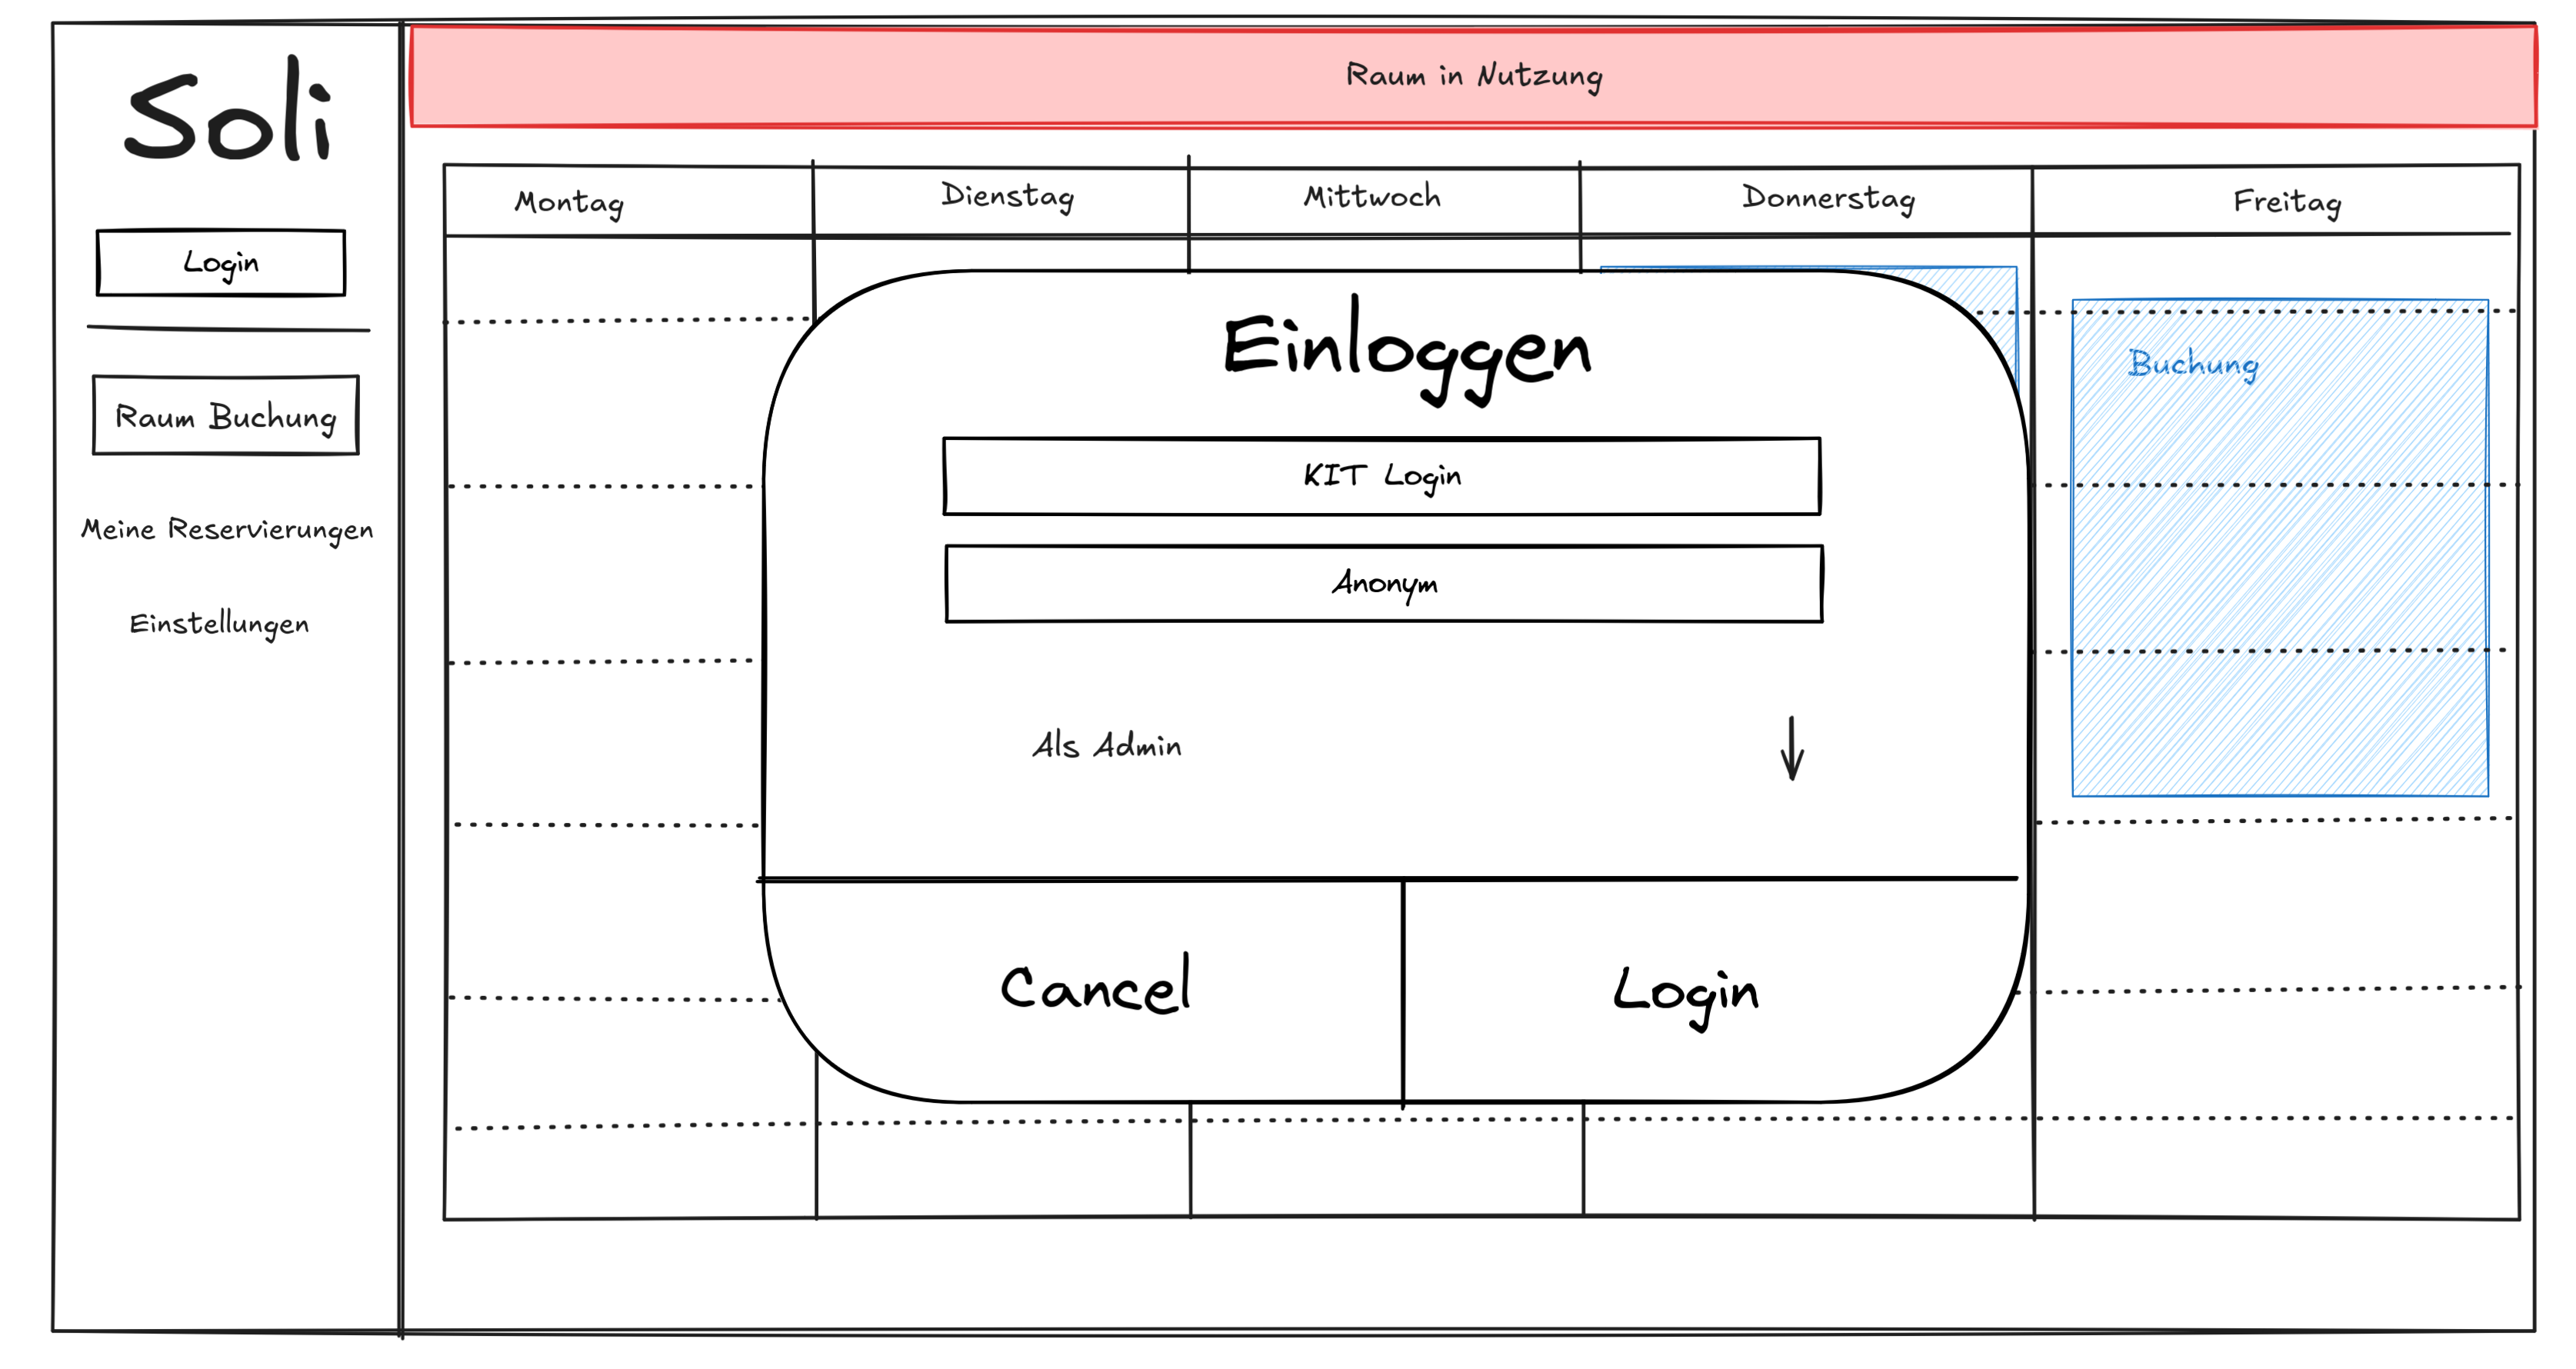
\includegraphics[width=0.65\textwidth]{pictures/figures/ui/anmeldungsseite}
        \label{fig:login}
    \end{figure}
\end{frame}

\begin{frame}
    \begin{figure}
        \centering
        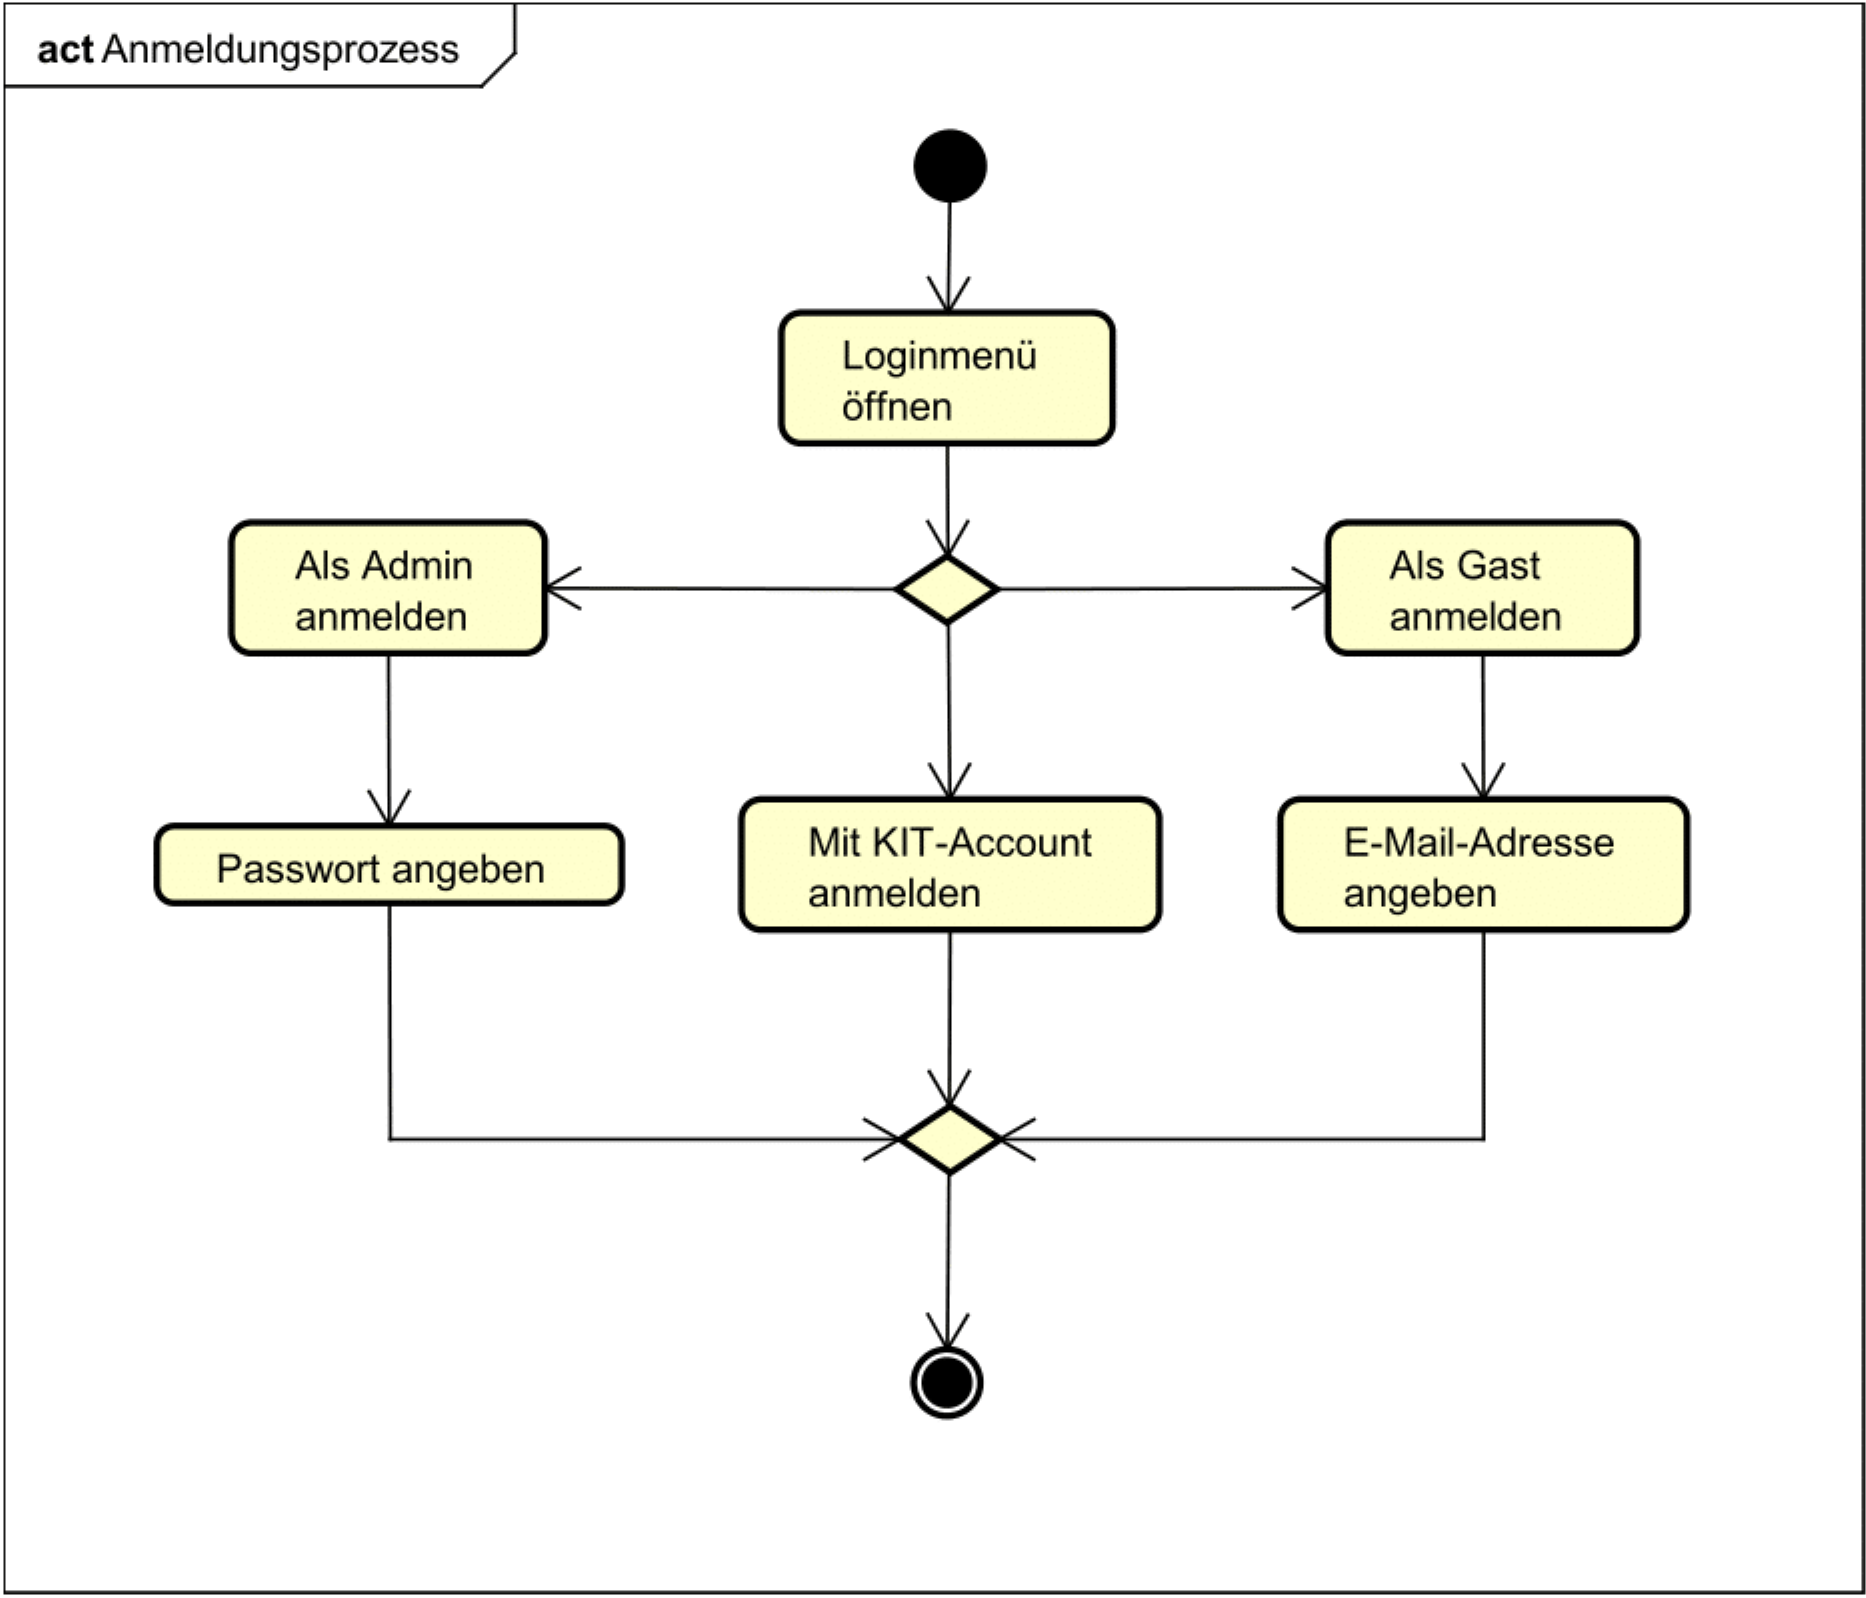
\includegraphics[width=0.55\textwidth]{pictures/figures/activity/anmeldeprozess}
        \caption{Mit der Anmeldung akzeptiert nun der Authentication Filter und der Großteil der Funktionalität ist nun zugänglich.}
        \label{fig:loginprozess}
    \end{figure}
\end{frame}

\begin{frame}{Kalenderansicht}
    \begin{figure}
        \centering
        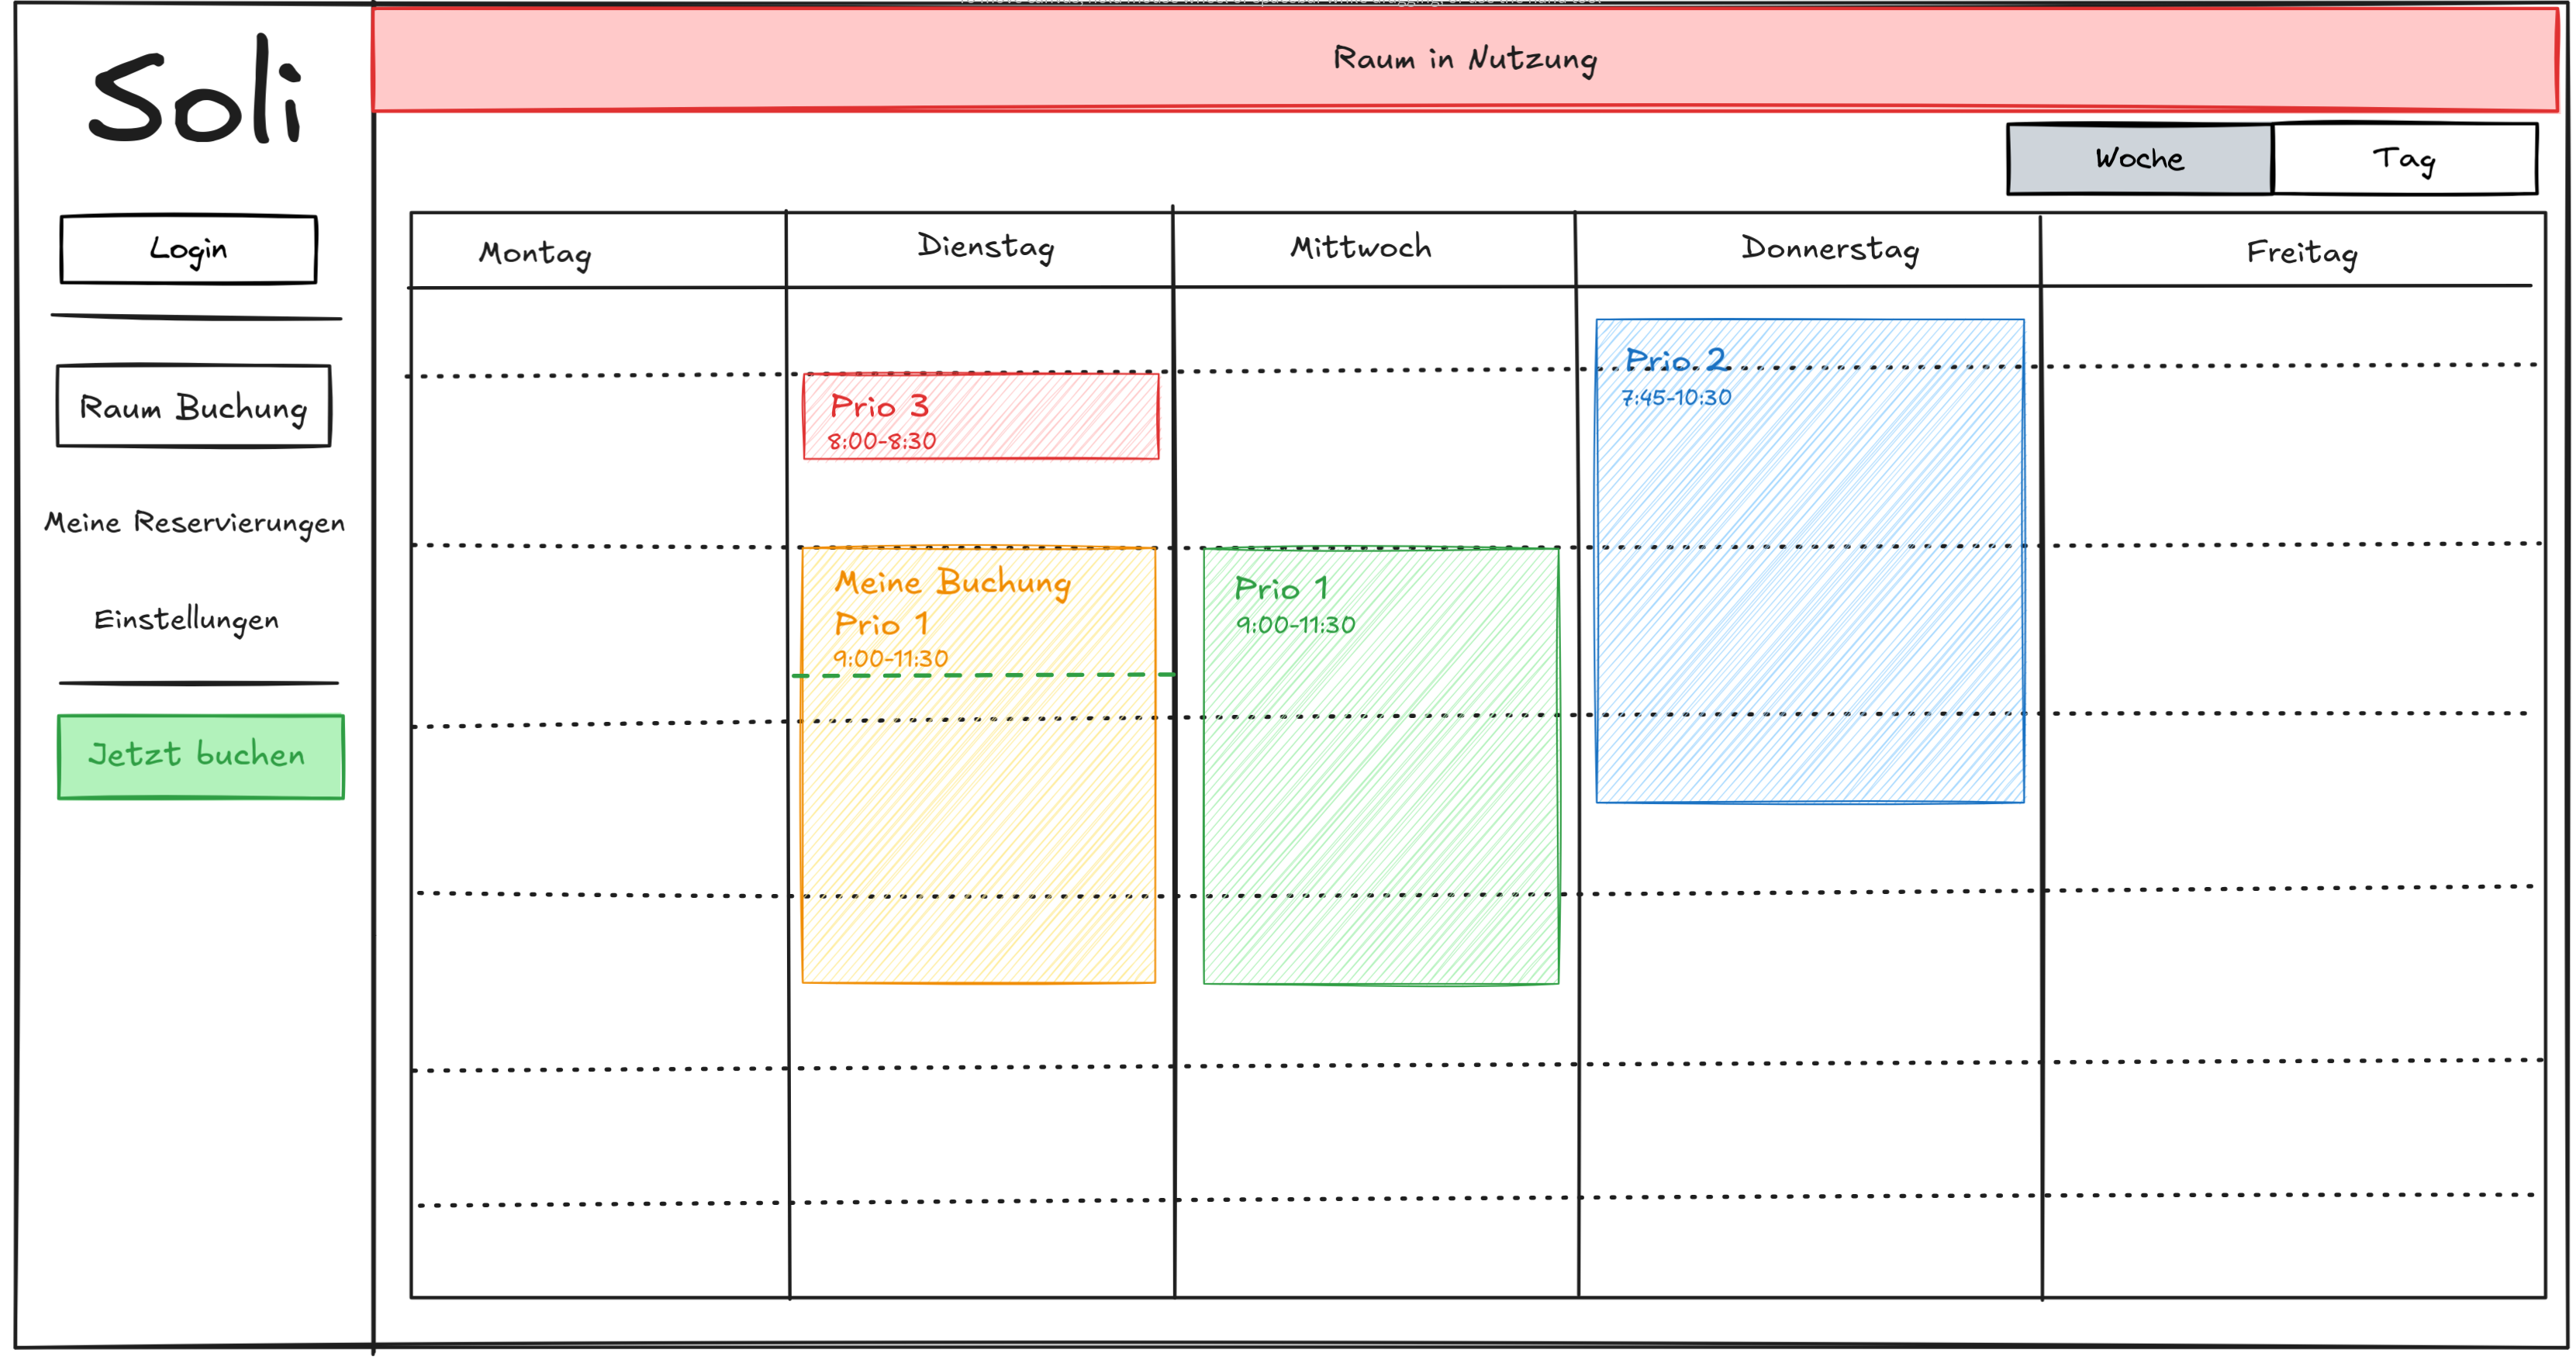
\includegraphics[width=0.65\textwidth]{pictures/figures/ui/startseite}
        \caption{Zeigt alle Termine an, die in der Datenbank gespeichert sind.}
        \label{fig:kalender}
    \end{figure}
\end{frame}

\begin{frame}
    \begin{figure}
        \centering
        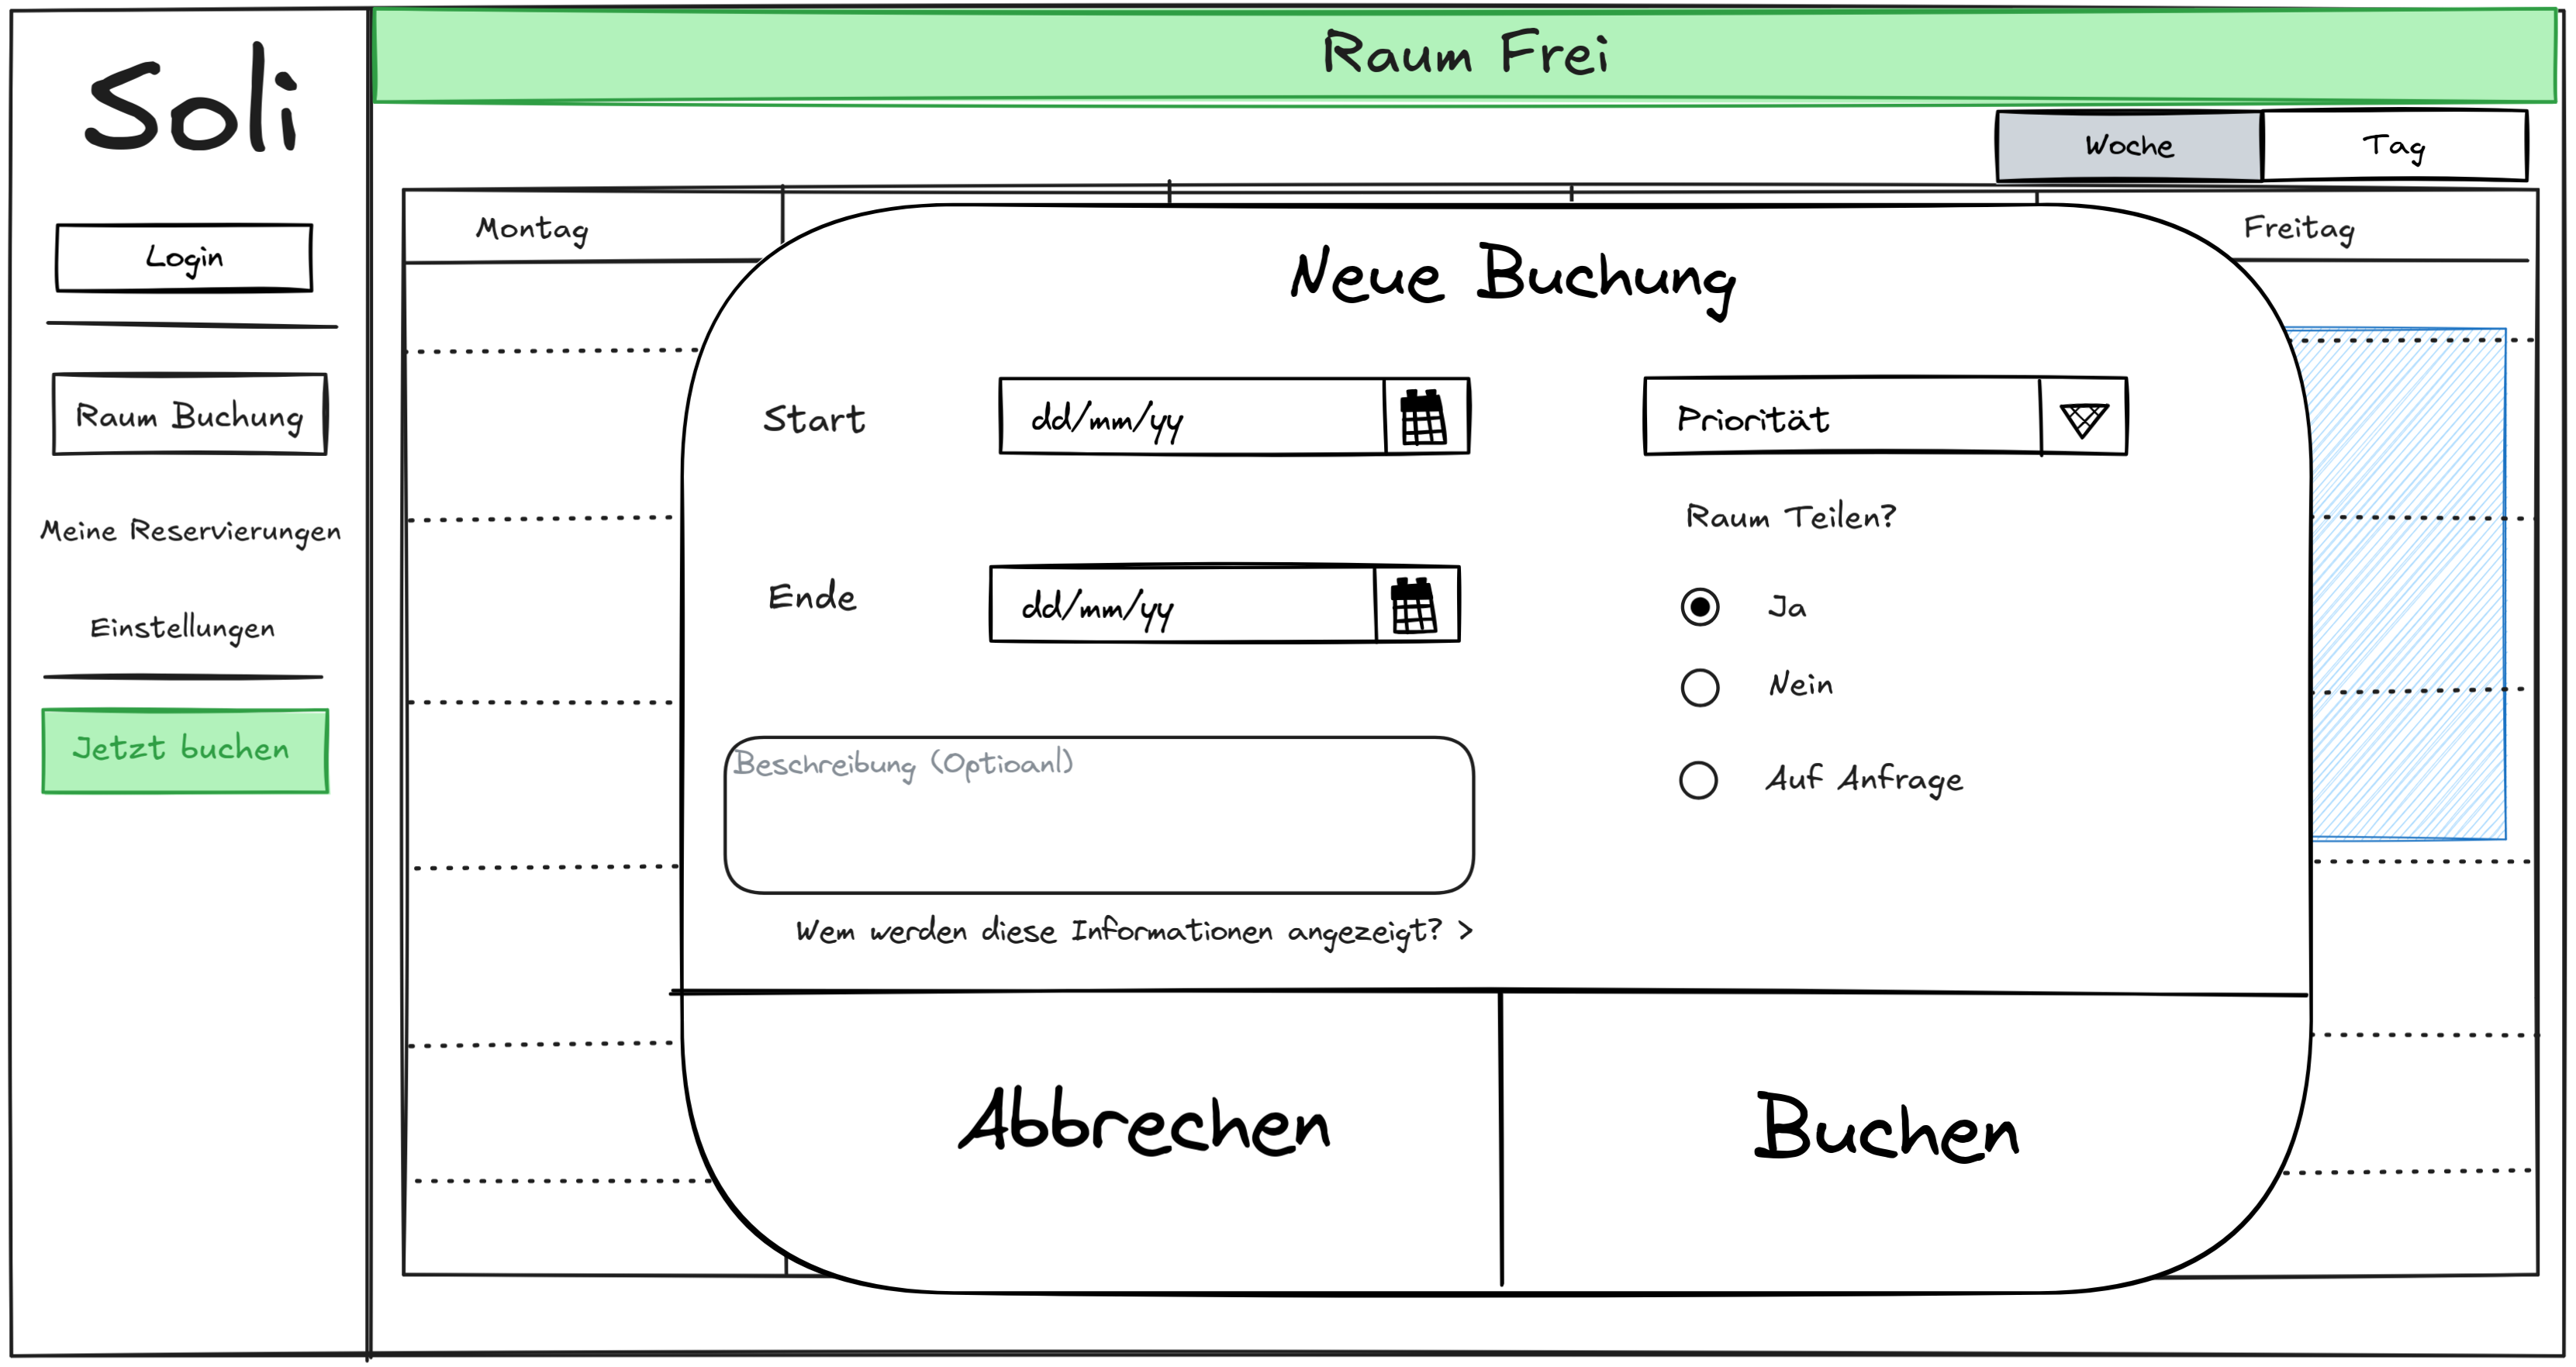
\includegraphics[width=0.8\textwidth]{pictures/figures/ui/buchungsdialog}
        \caption{Diese Ansicht wird über die Kalenderansicht erreicht.}
        \label{fig:terminerstellen}
    \end{figure}
\end{frame}

\begin{frame}[plain]
    \begin{figure}
        \centering
        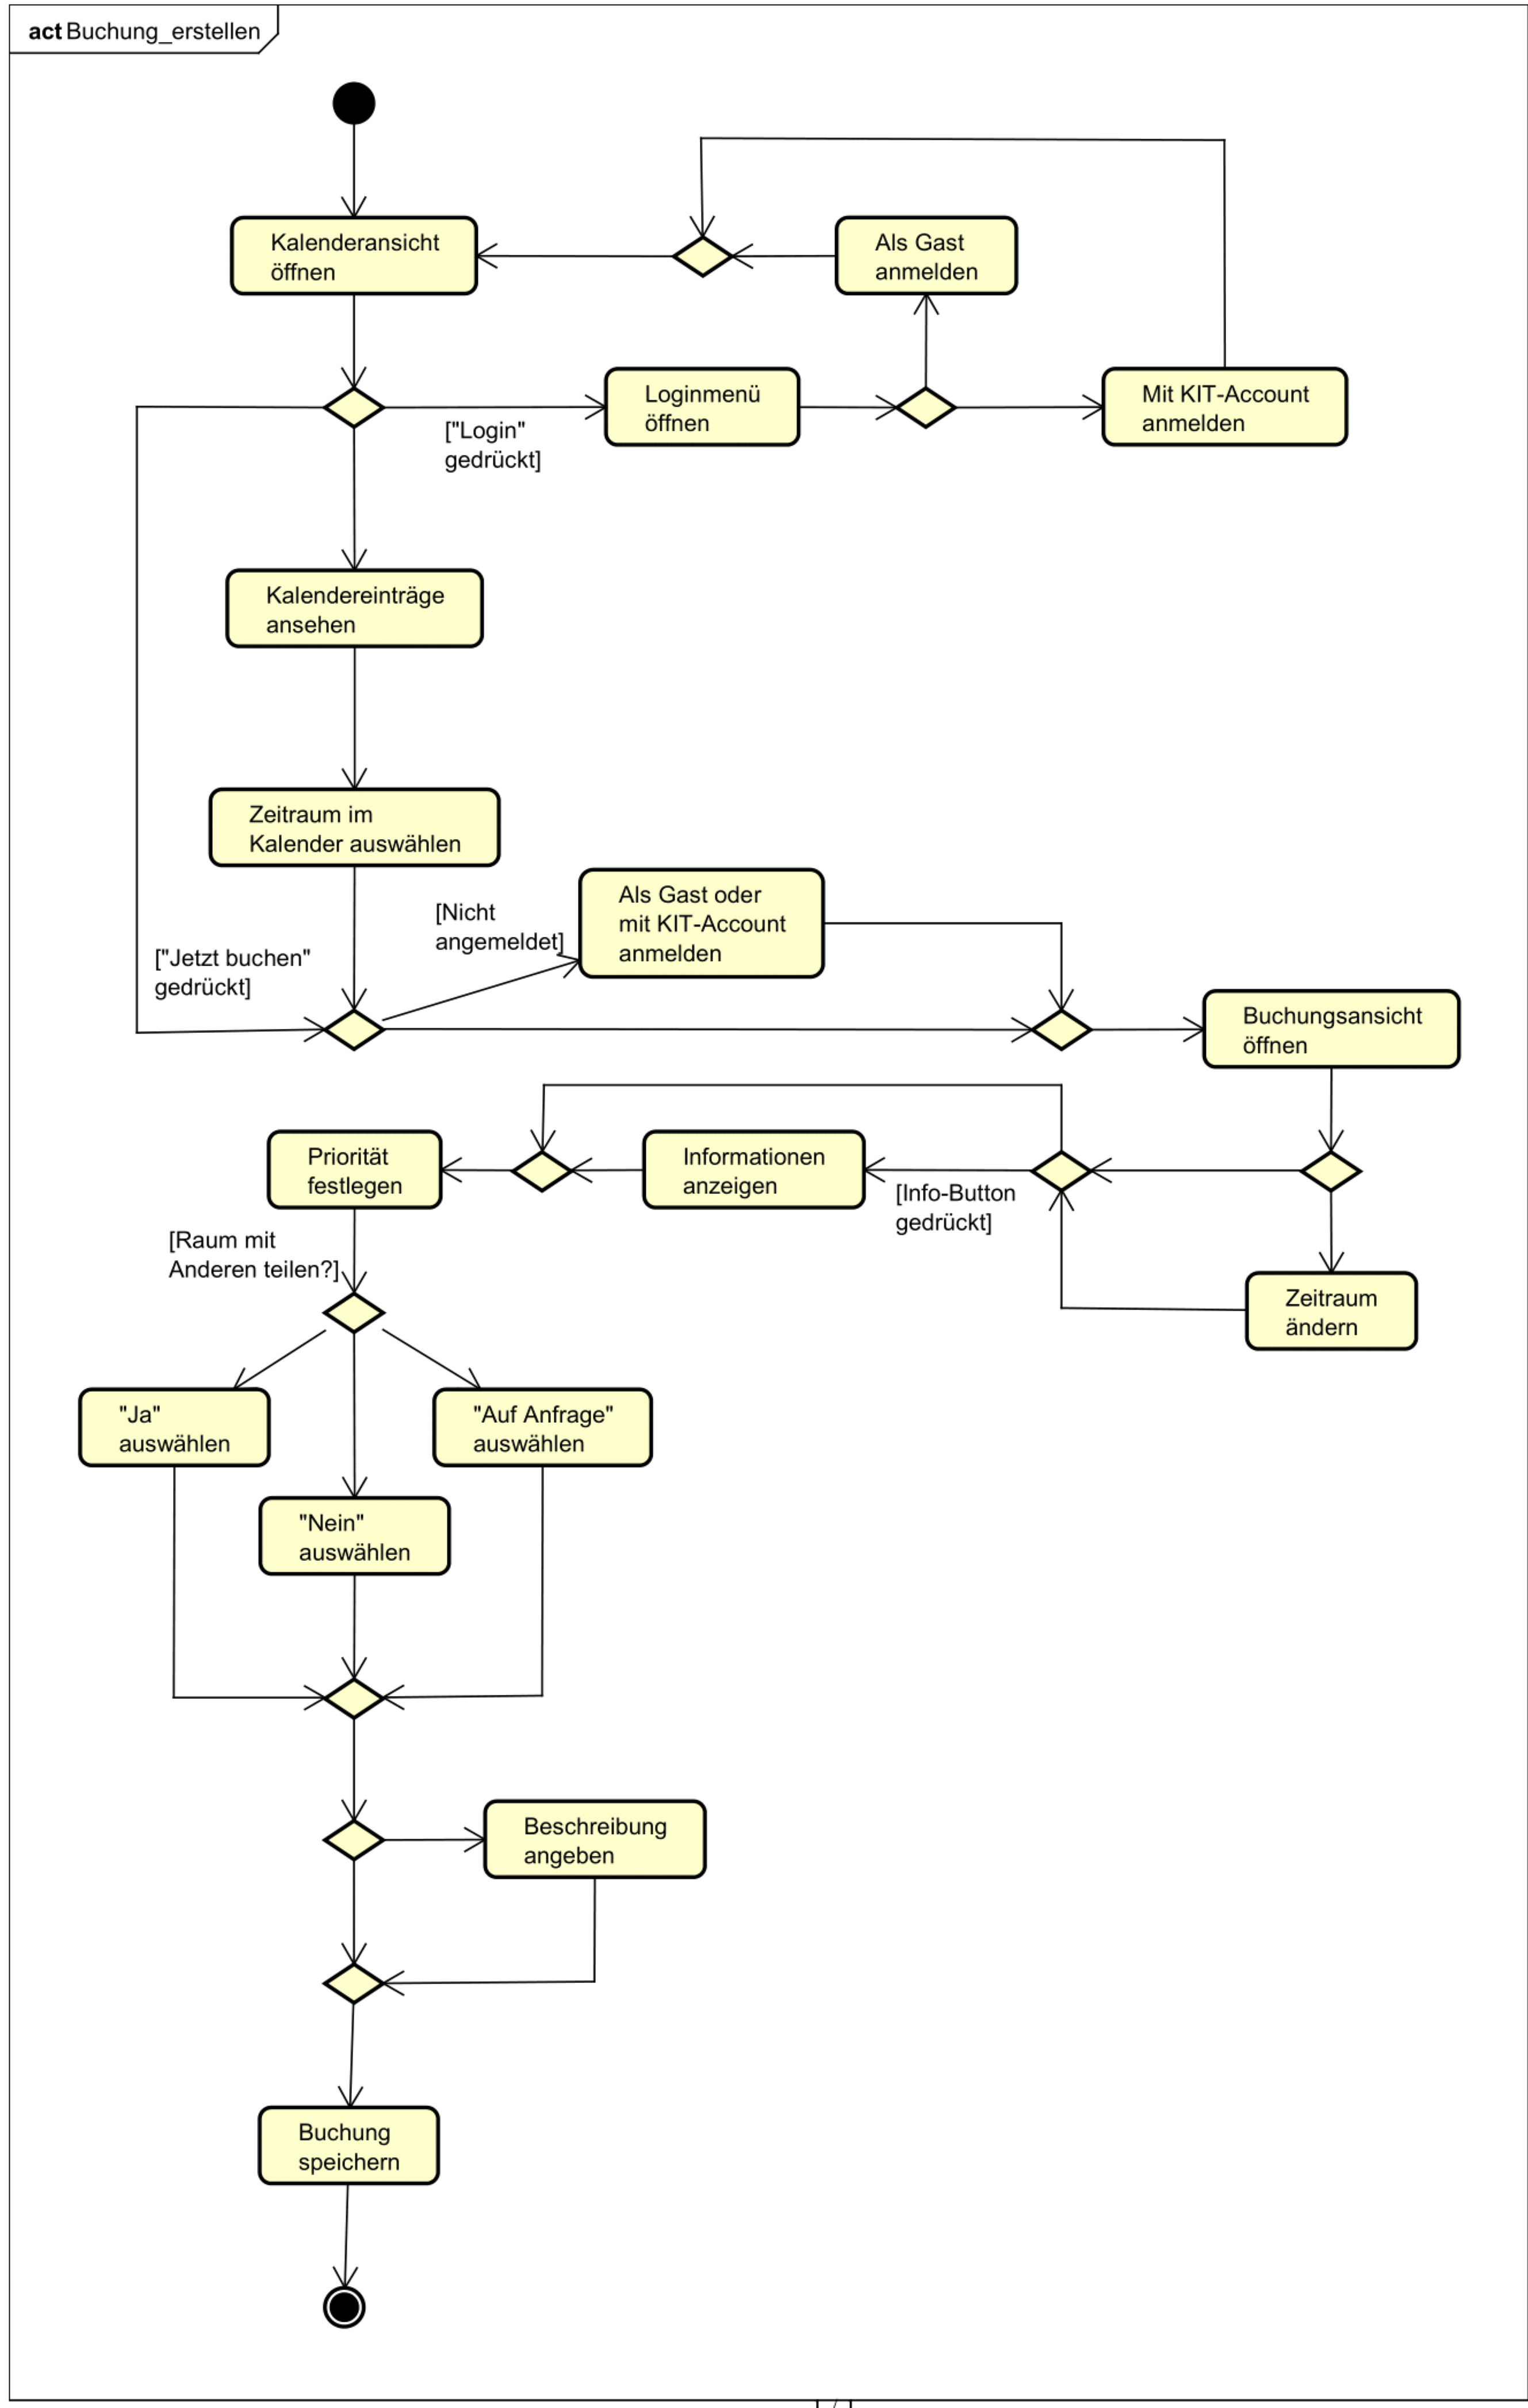
\includegraphics[width=0.35\textwidth]{pictures/figures/activity/buchungerstellen}
        \caption{Der Termin wird in der Datenbank gespeichert und ist nun in der Kalenderansicht sichtbar.}
        \label{fig:terminerstellenprozess}
    \end{figure}
\end{frame}

\begin{frame}[plain]
    \begin{figure}
        \centering
        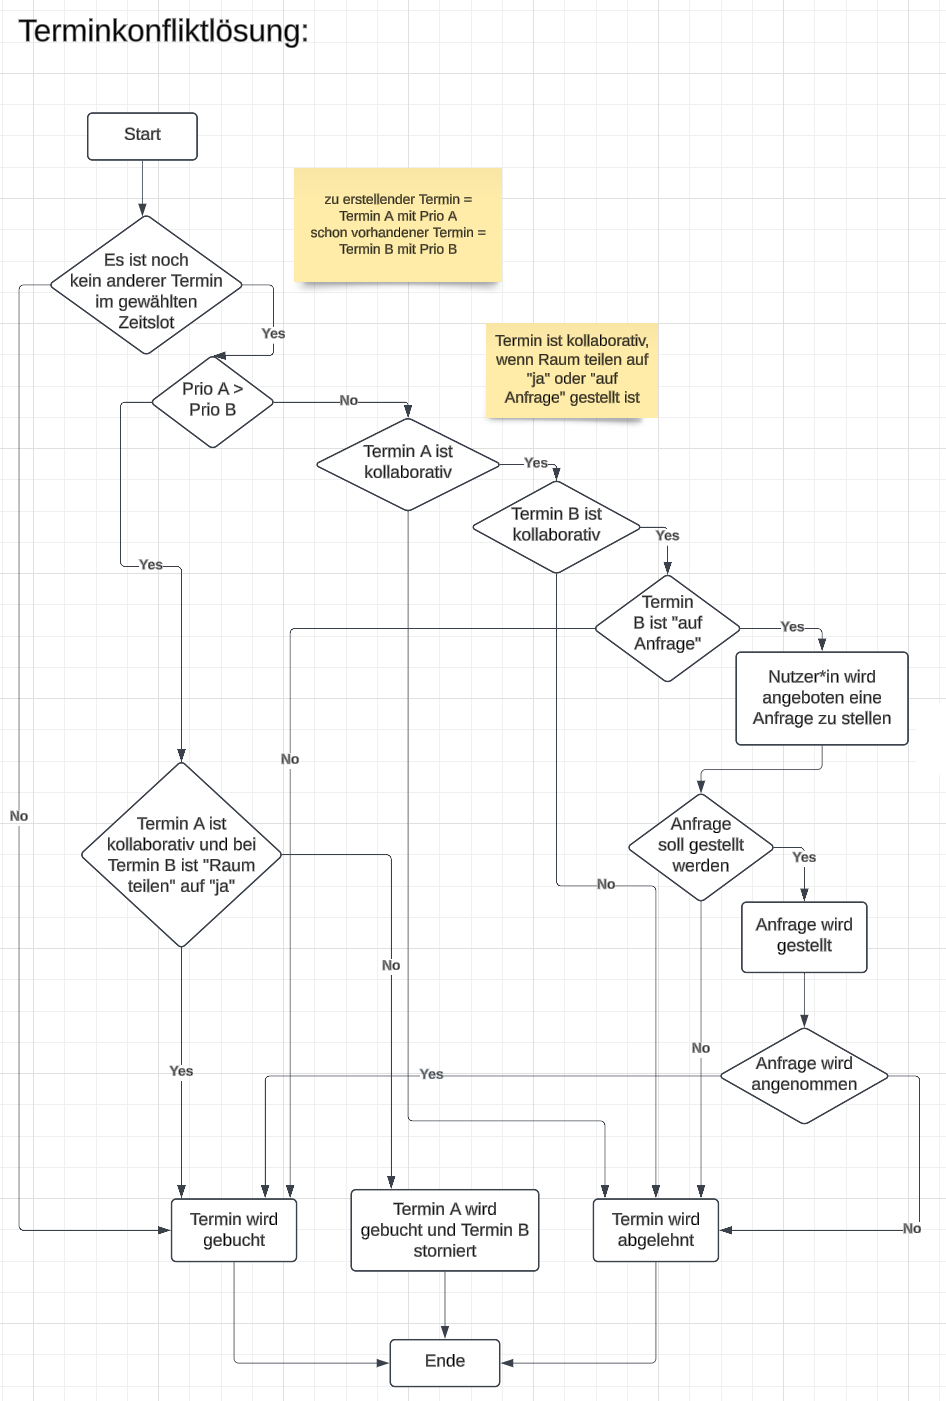
\includegraphics[width=0.4\textwidth]{pictures/figures/activity/terminkonfliktloesung}
        \label{fig:terminkonflikt}
    \end{figure}
\end{frame}

\begin{frame}[plain]
    \begin{figure}
        \centering
        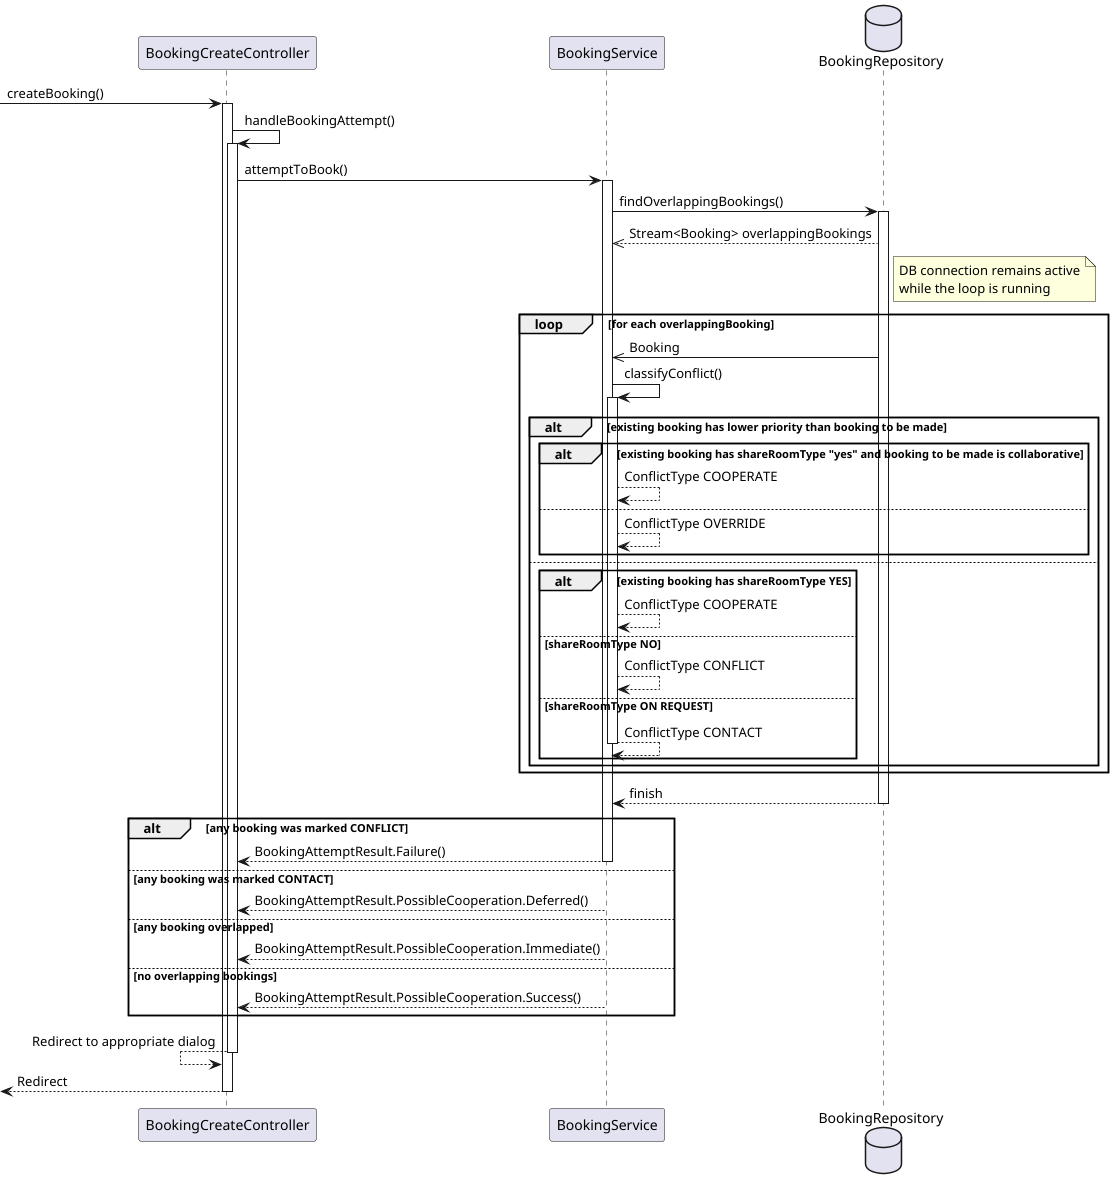
\includegraphics[width=0.55\textwidth]{pictures/figures/activity/SequenzdiagrammBuchungErstellen}
        \label{fig:terminerstellensequenz}
    \end{figure}
\end{frame}

\begin{frame}{Terminübersicht}
    \begin{figure}
        \centering
        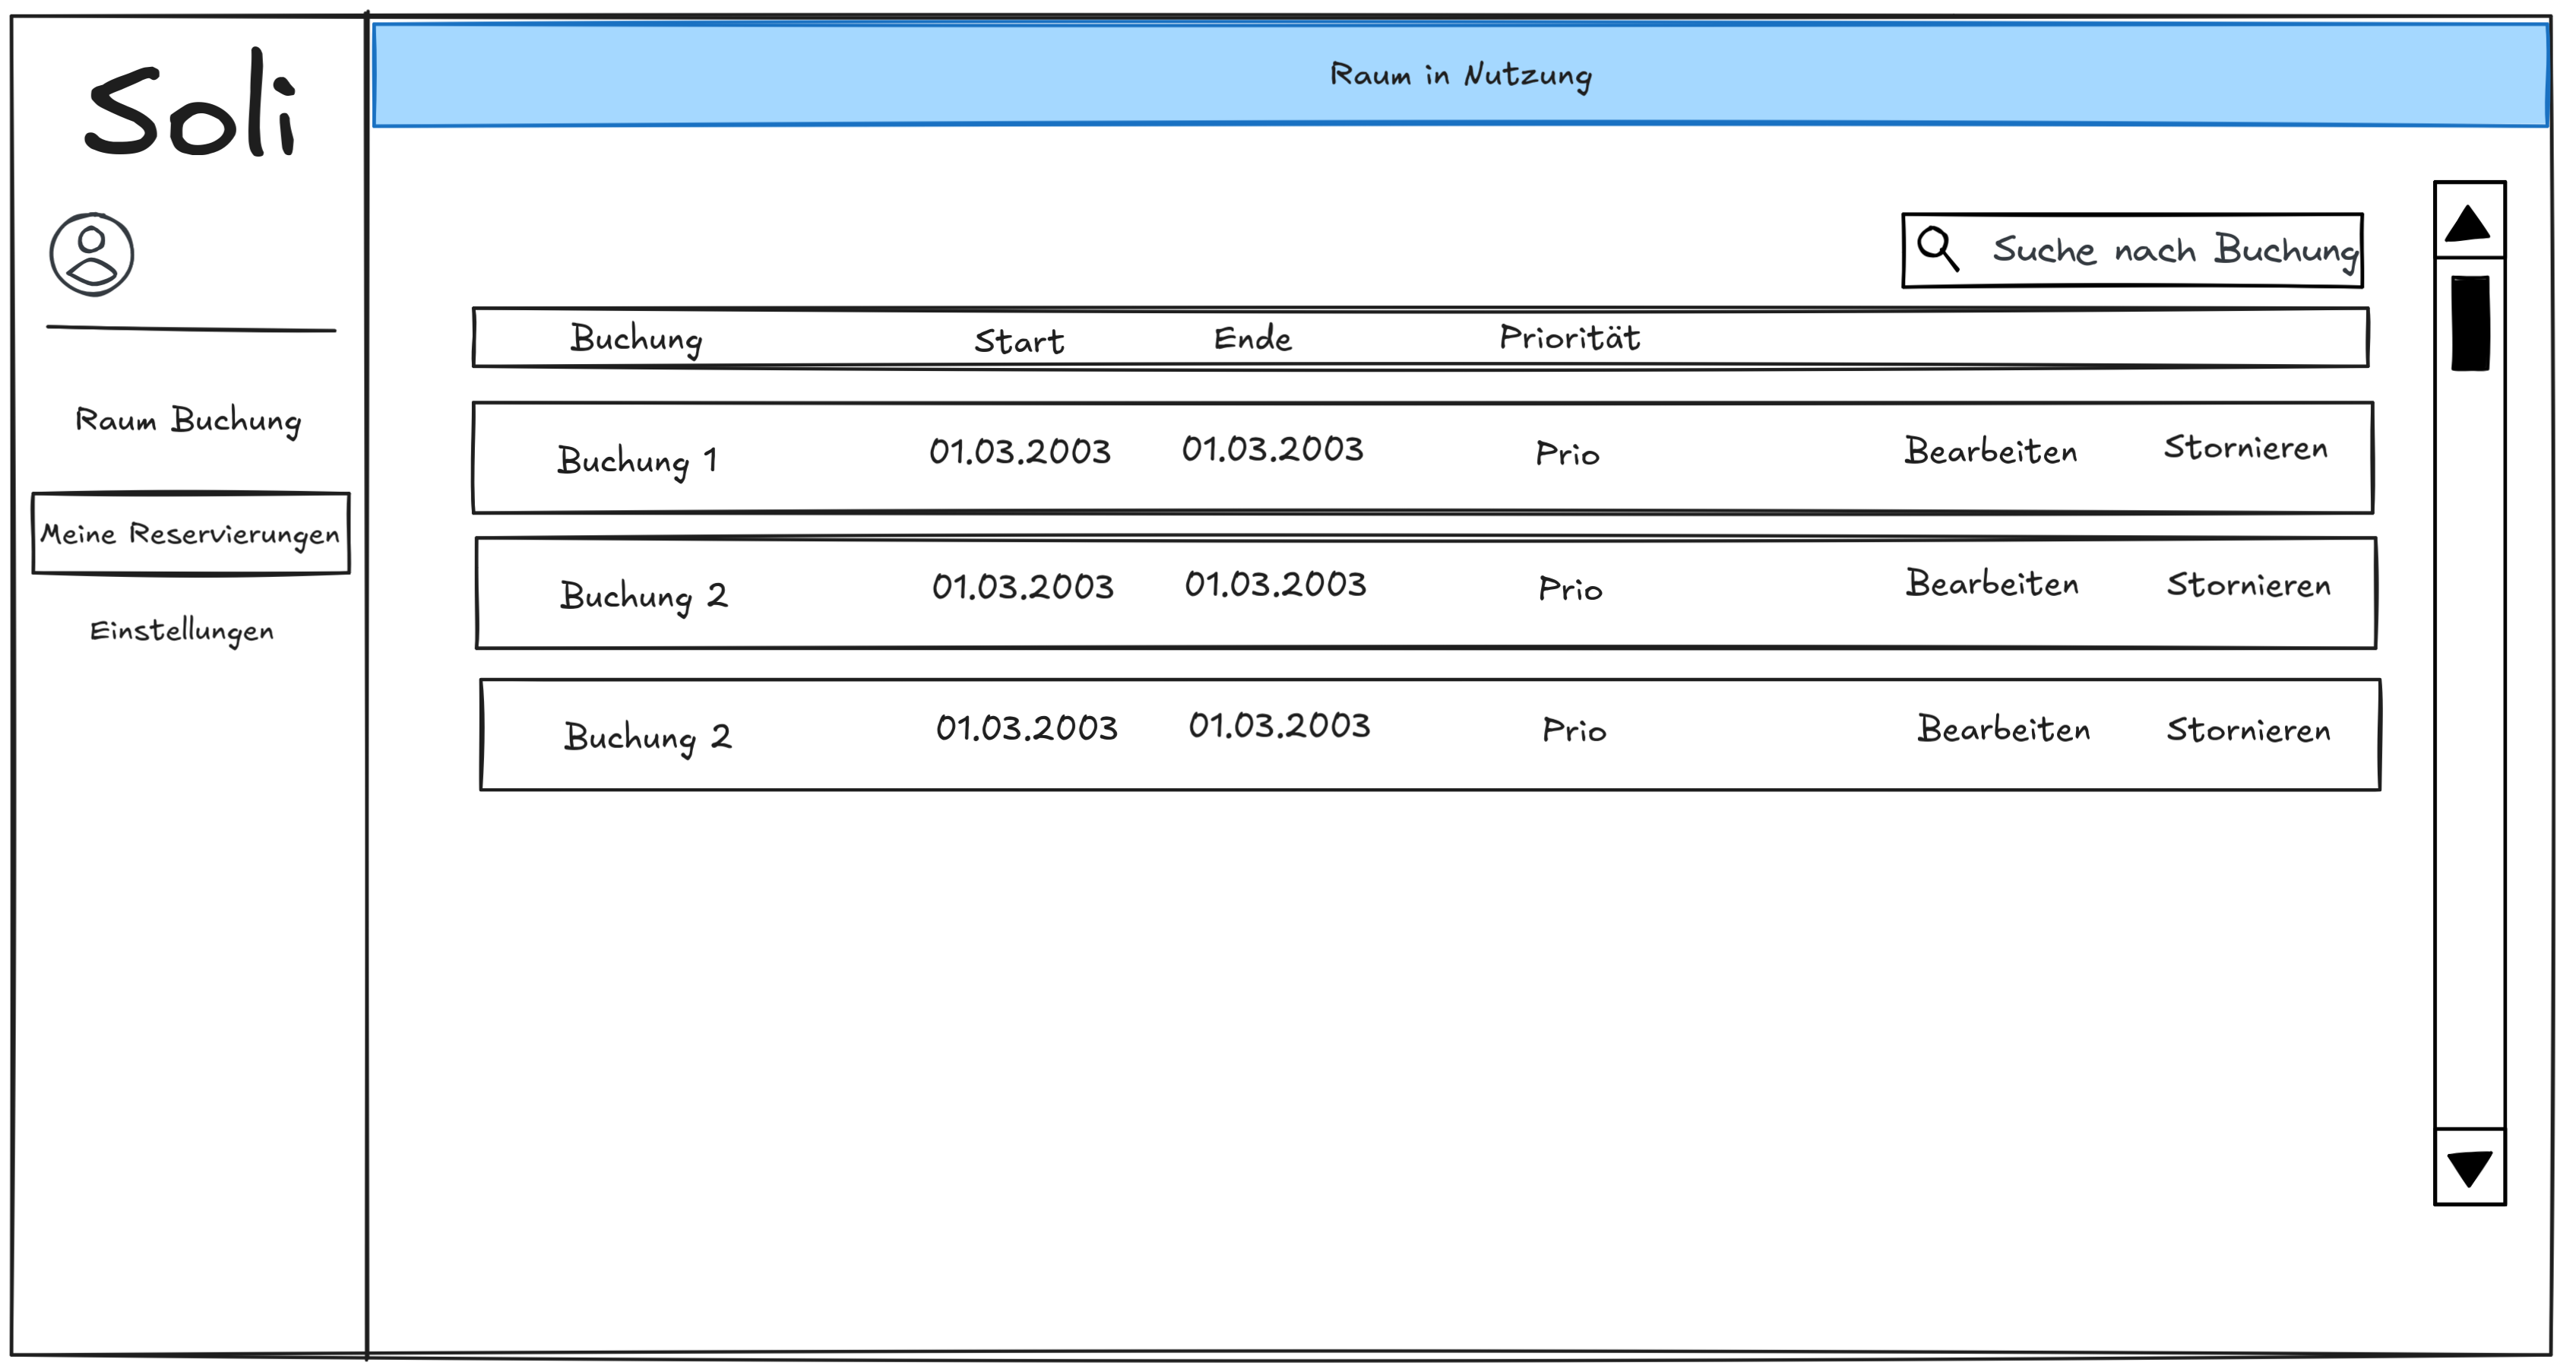
\includegraphics[width=0.65\textwidth]{pictures/figures/ui/reservierungsuebersicht}
        \caption{Zeigt alle Termine an, die der/die Nutzende erstellt hat.}
        \label{fig:terminuebersicht}
    \end{figure}
\end{frame}

\begin{frame}[plain]
    \begin{figure}
        \centering
        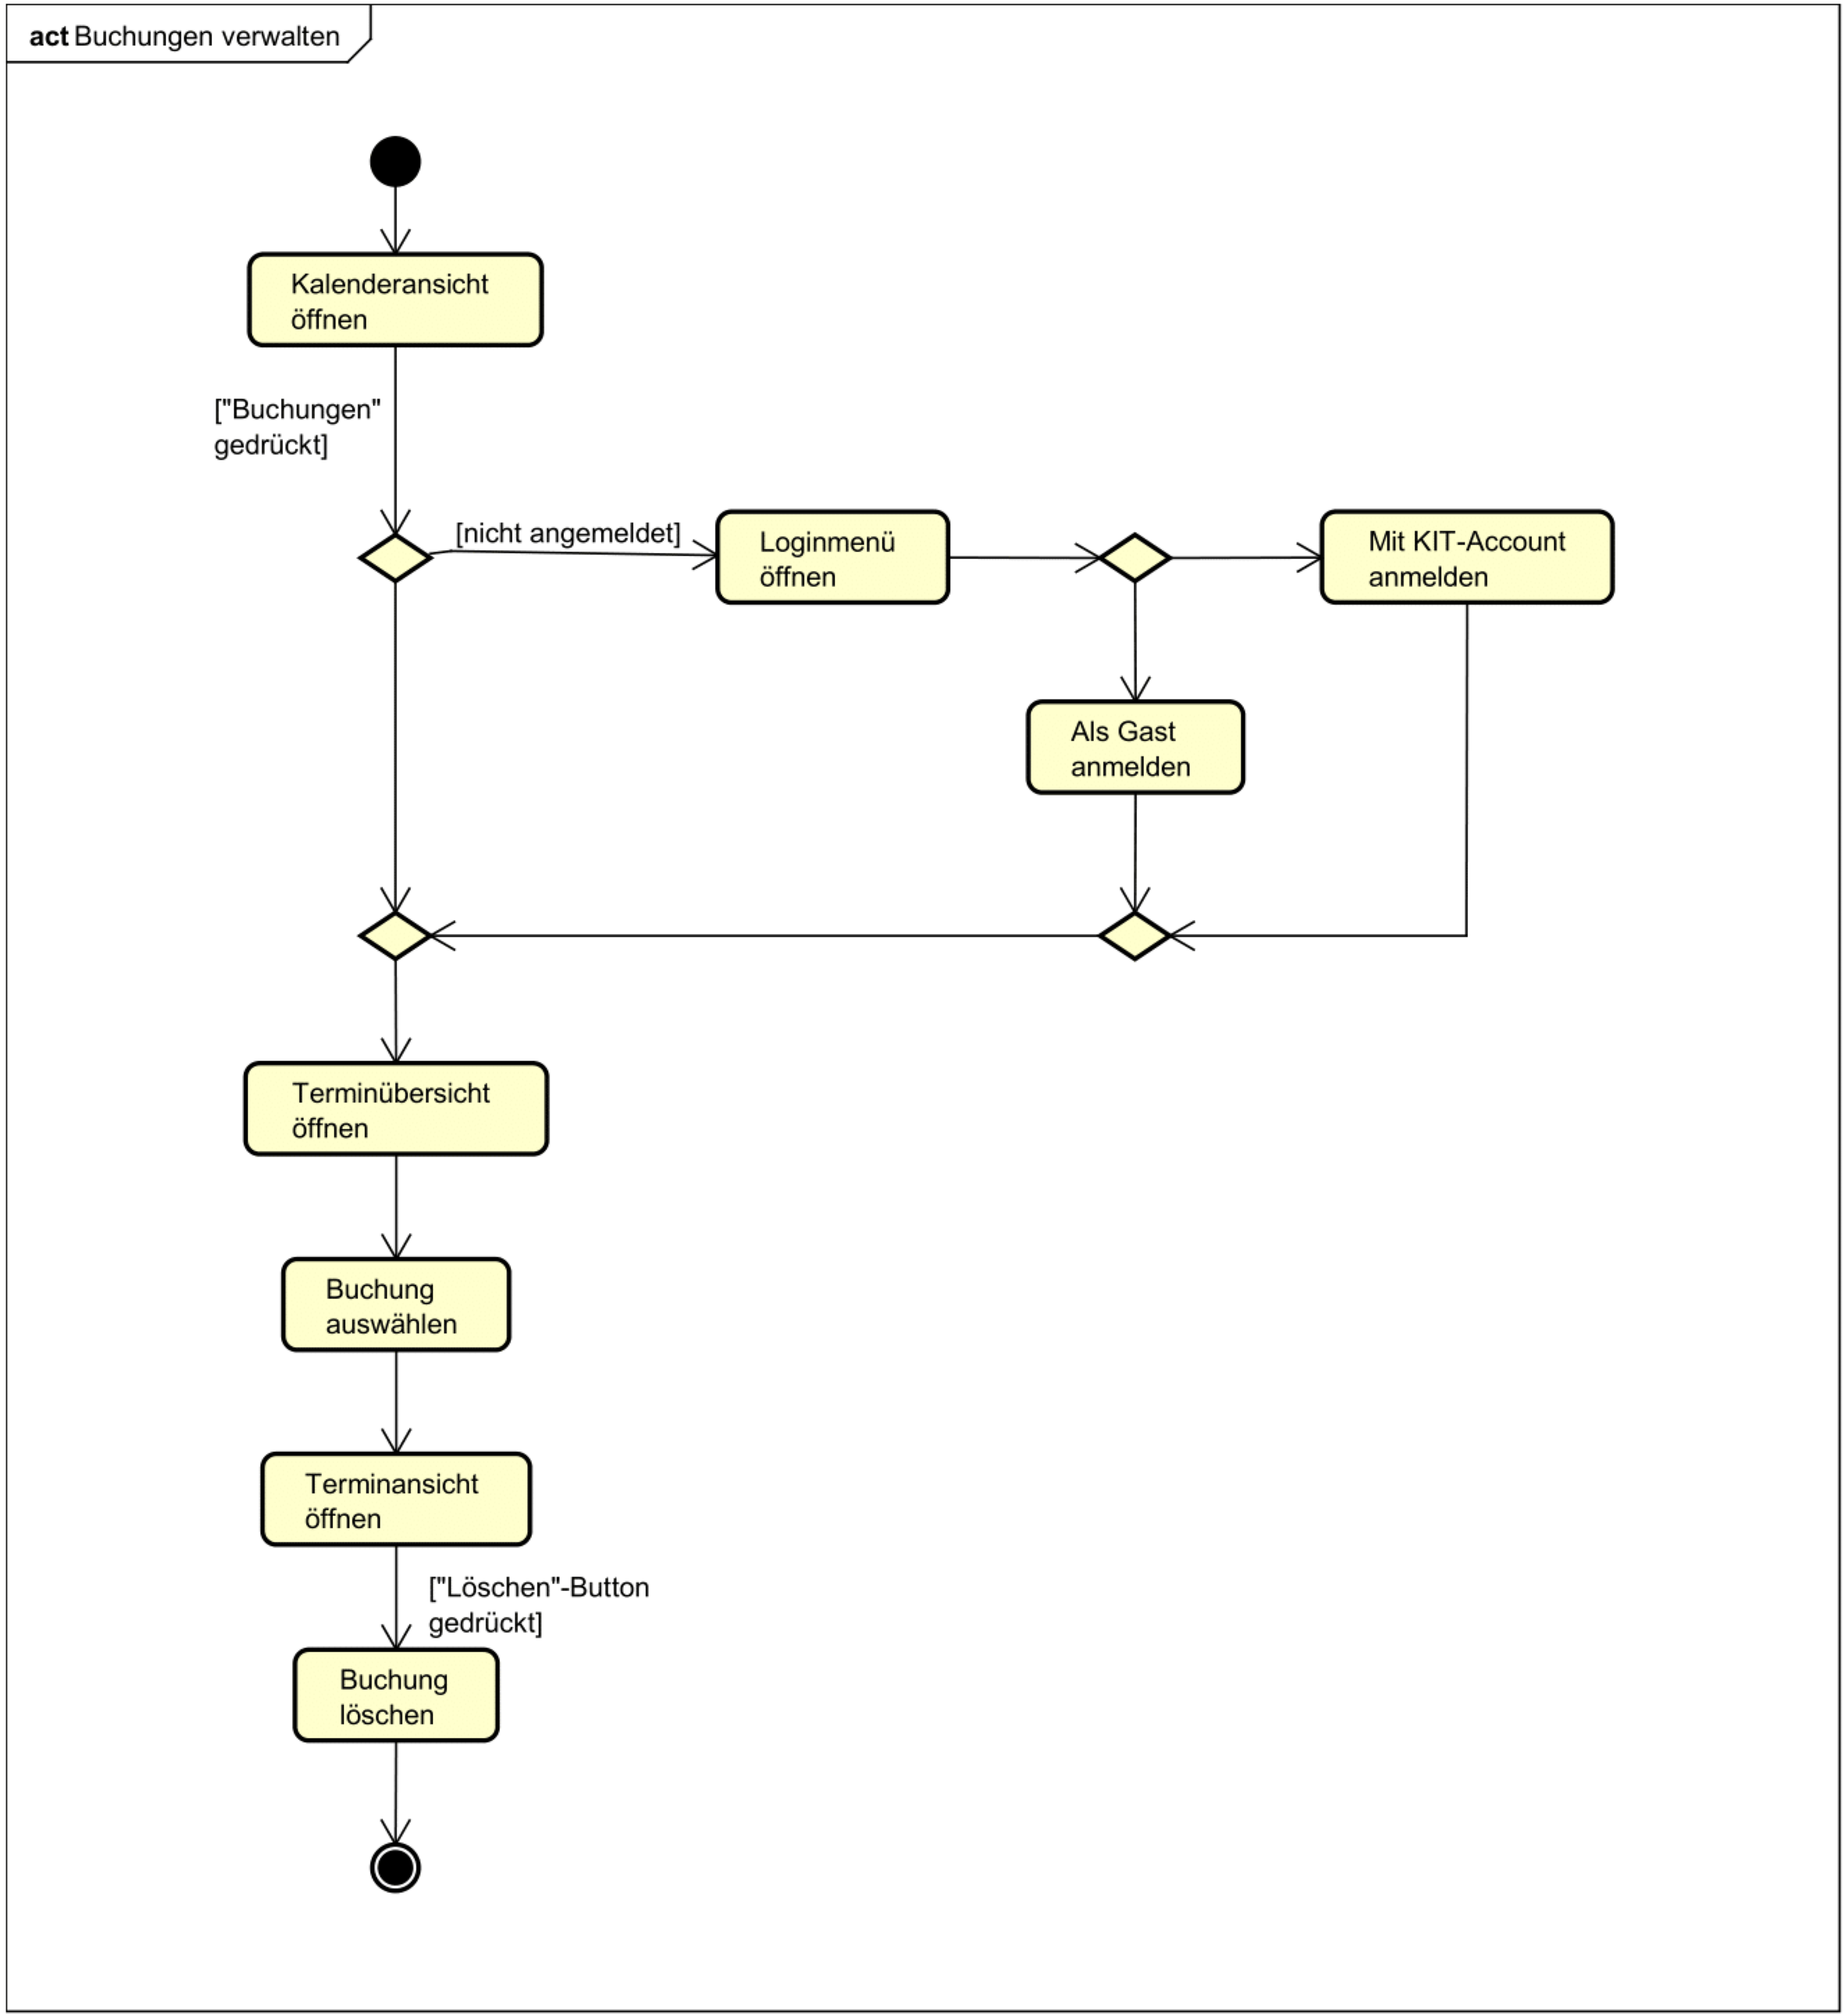
\includegraphics[width=0.55\textwidth]{pictures/figures/activity/buchungverwalten}
        \label{fig:terminuebersichtprozess}
    \end{figure}
\end{frame}

\begin{frame}{Terminansicht}
    \begin{figure}
        \centering
        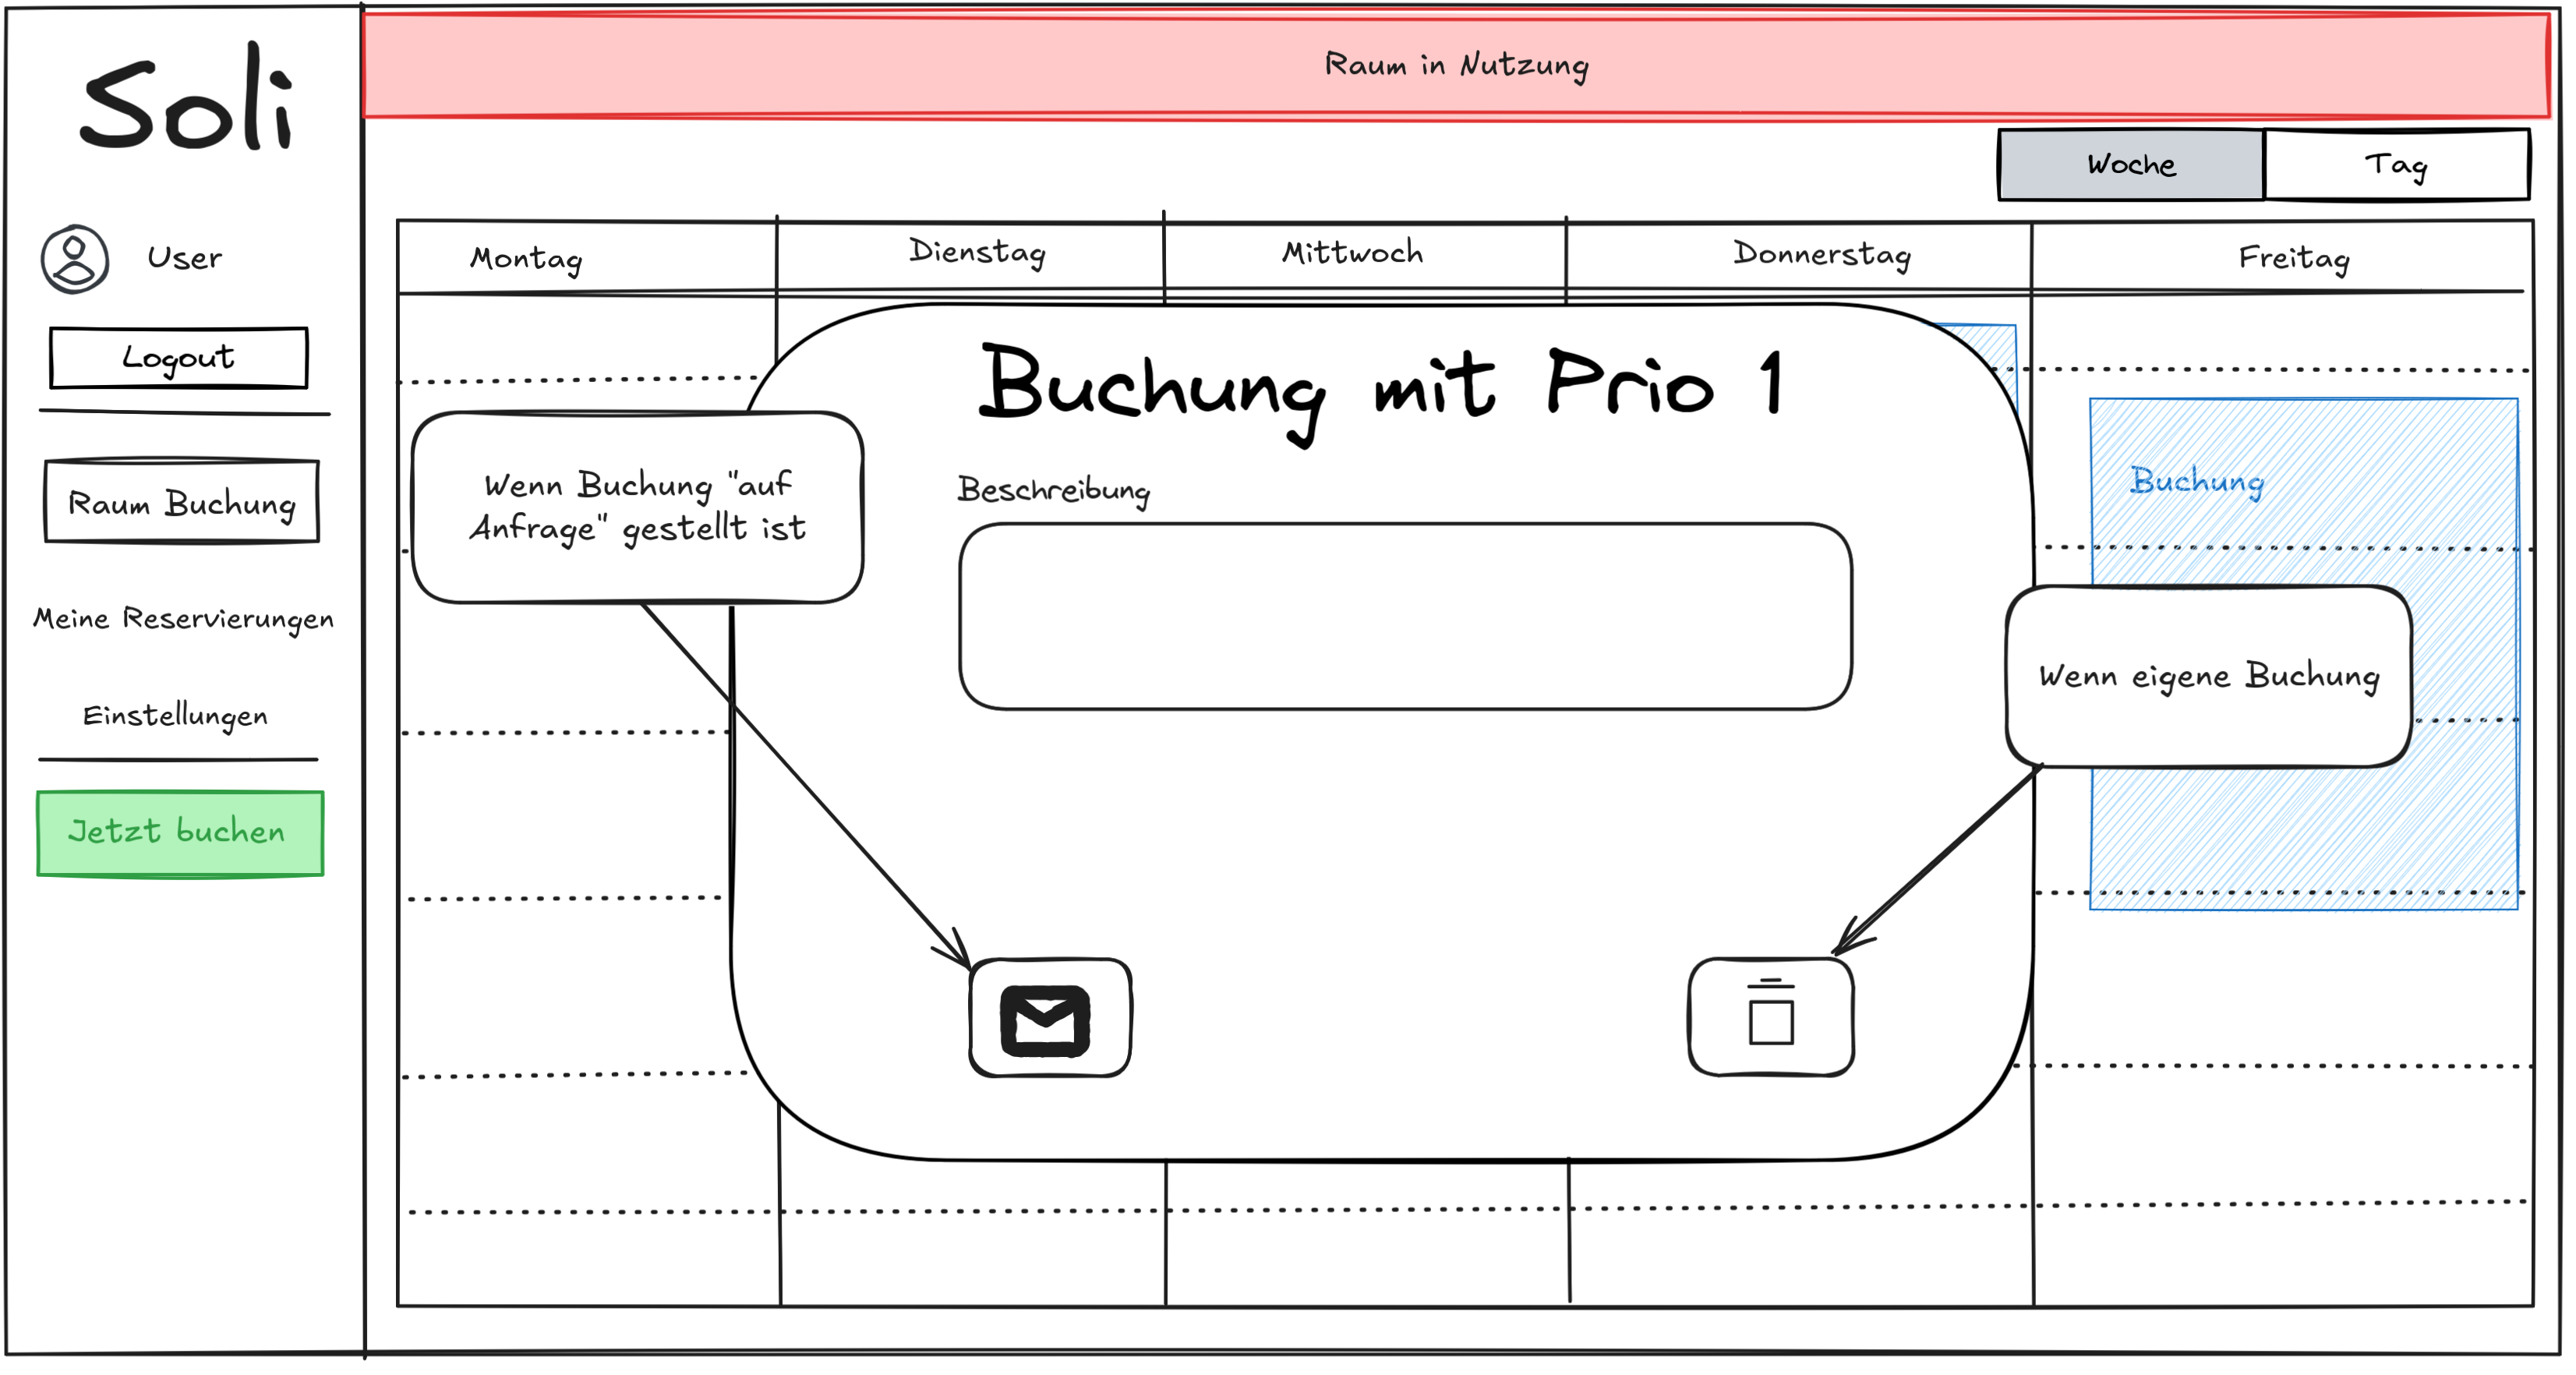
\includegraphics[width=0.65\textwidth]{pictures/figures/ui/reservierunginkalendar}
        \caption{Zeigt alle Informationen des Termins an.}
        \label{fig:terminansicht}
    \end{figure}
\end{frame}

\begin{frame}[plain]
    \begin{figure}
        \centering
        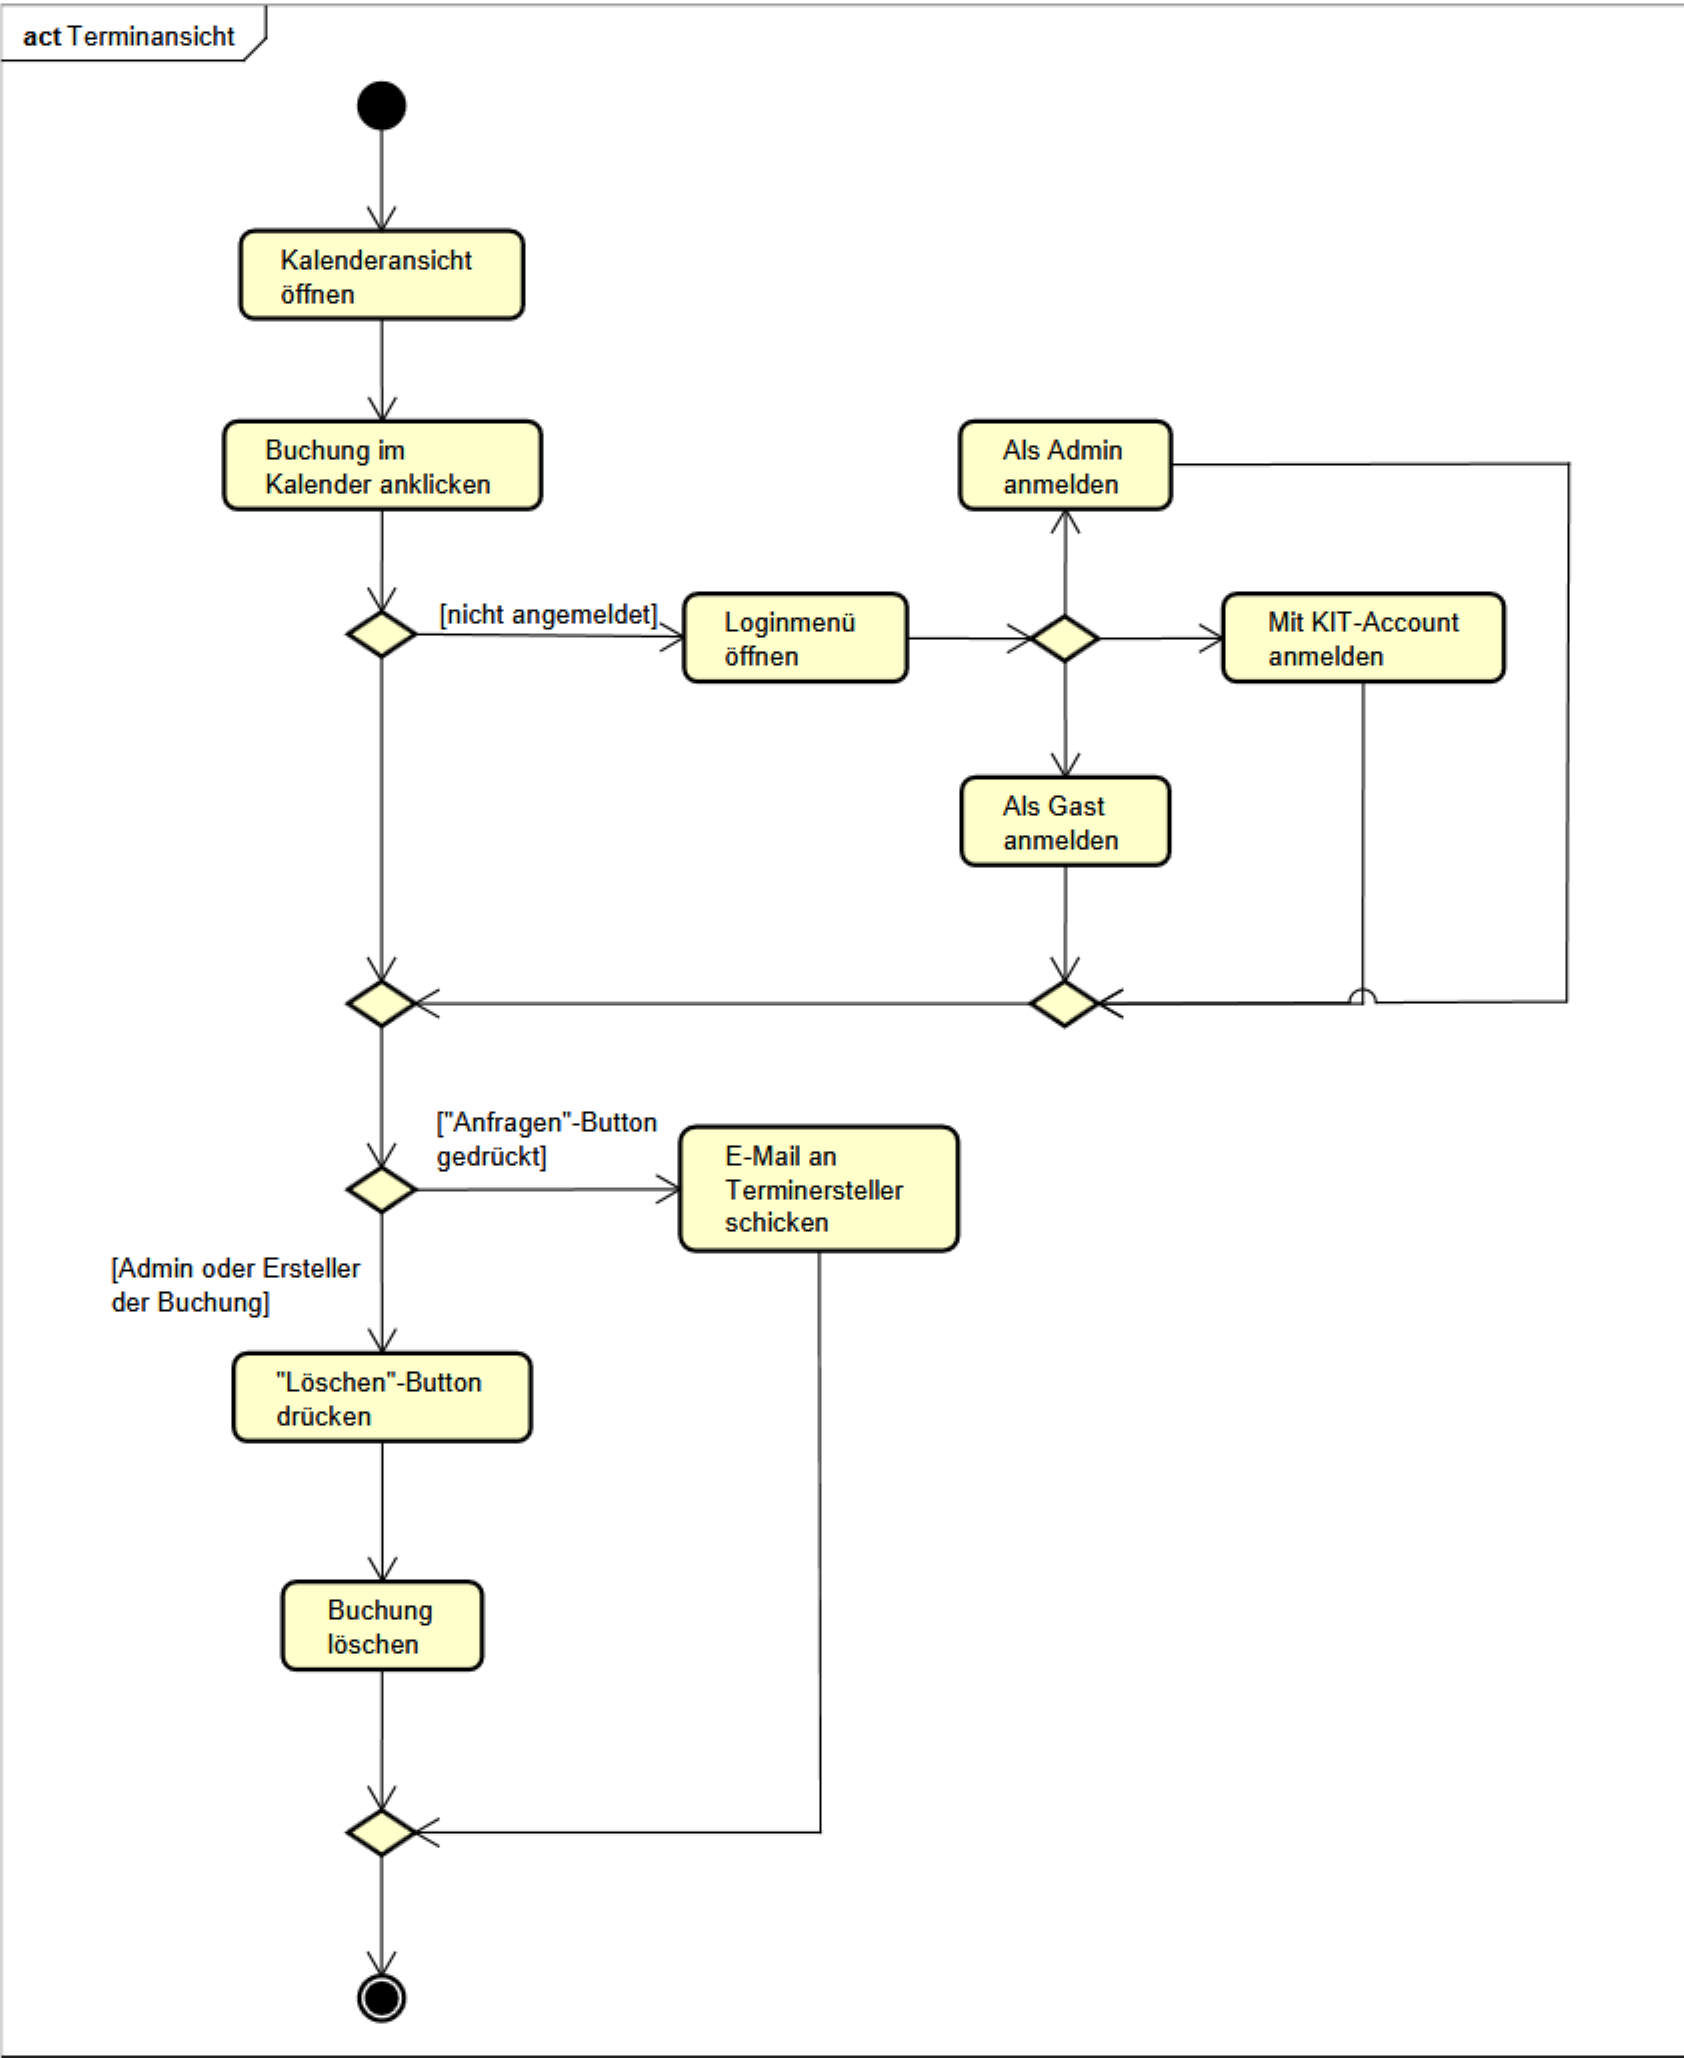
\includegraphics[width=0.49\textwidth]{pictures/figures/activity/terminansicht}
        \label{fig:terminansichtprozess}
    \end{figure}
\end{frame}

\begin{frame}{Checkout}
    \begin{minipage}{0.65\textwidth}
        \centering
        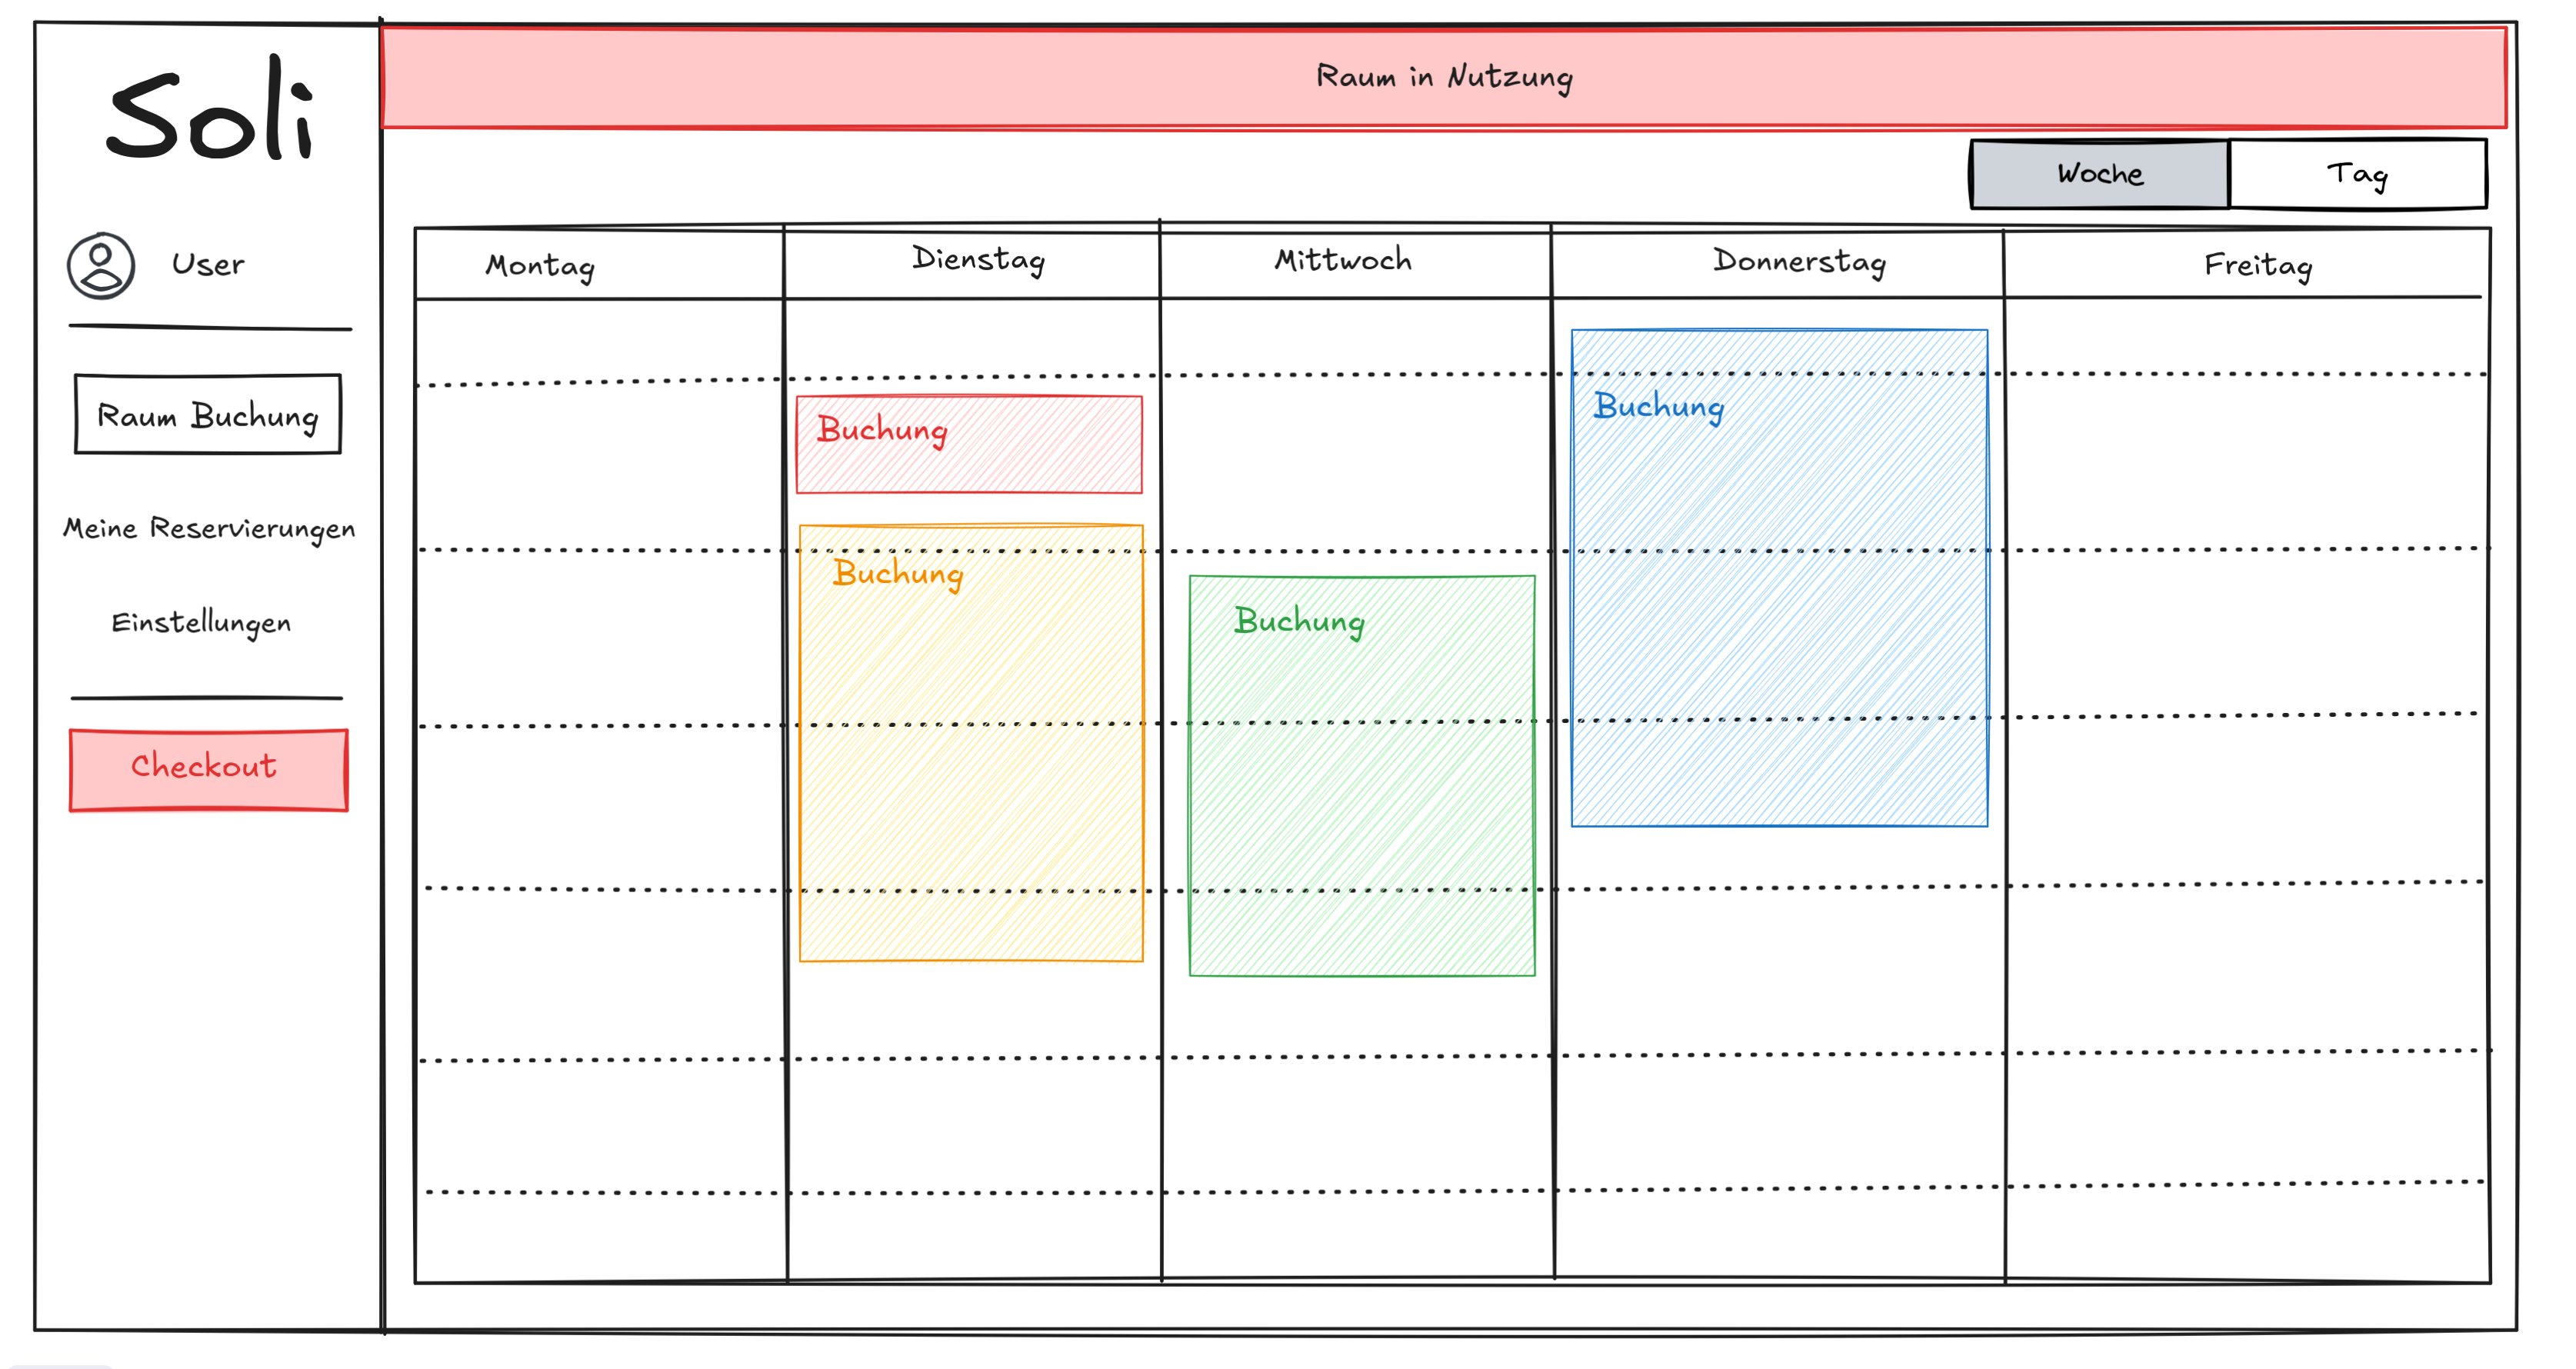
\includegraphics[width=\textwidth]{pictures/figures/ui/checkout}
        \label{fig:checkout}
    \end{minipage}
    \begin{minipage}{0.25\textwidth}
        \centering
        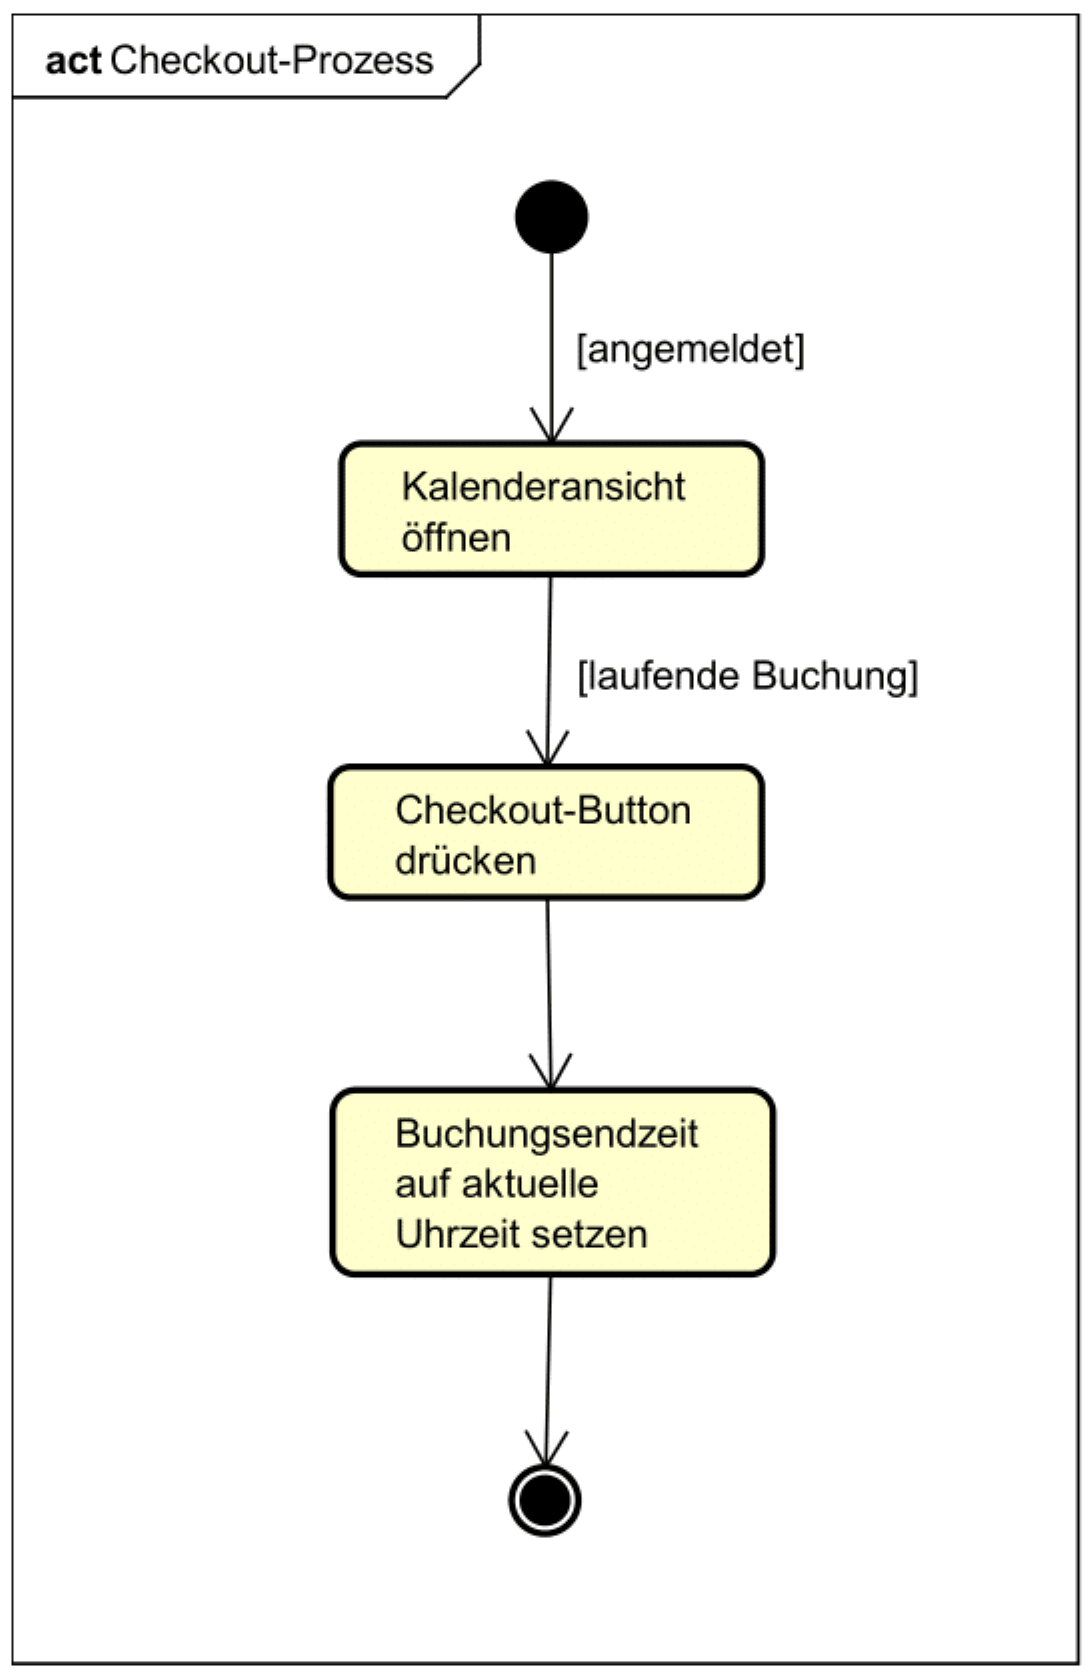
\includegraphics[width=\textwidth]{pictures/figures/activity/checkoutprozess}
        \label{fig:checkoutprozess}
    \end{minipage}
\end{frame}

\begin{frame}{Kontenliste}
    \begin{figure}
        \centering
        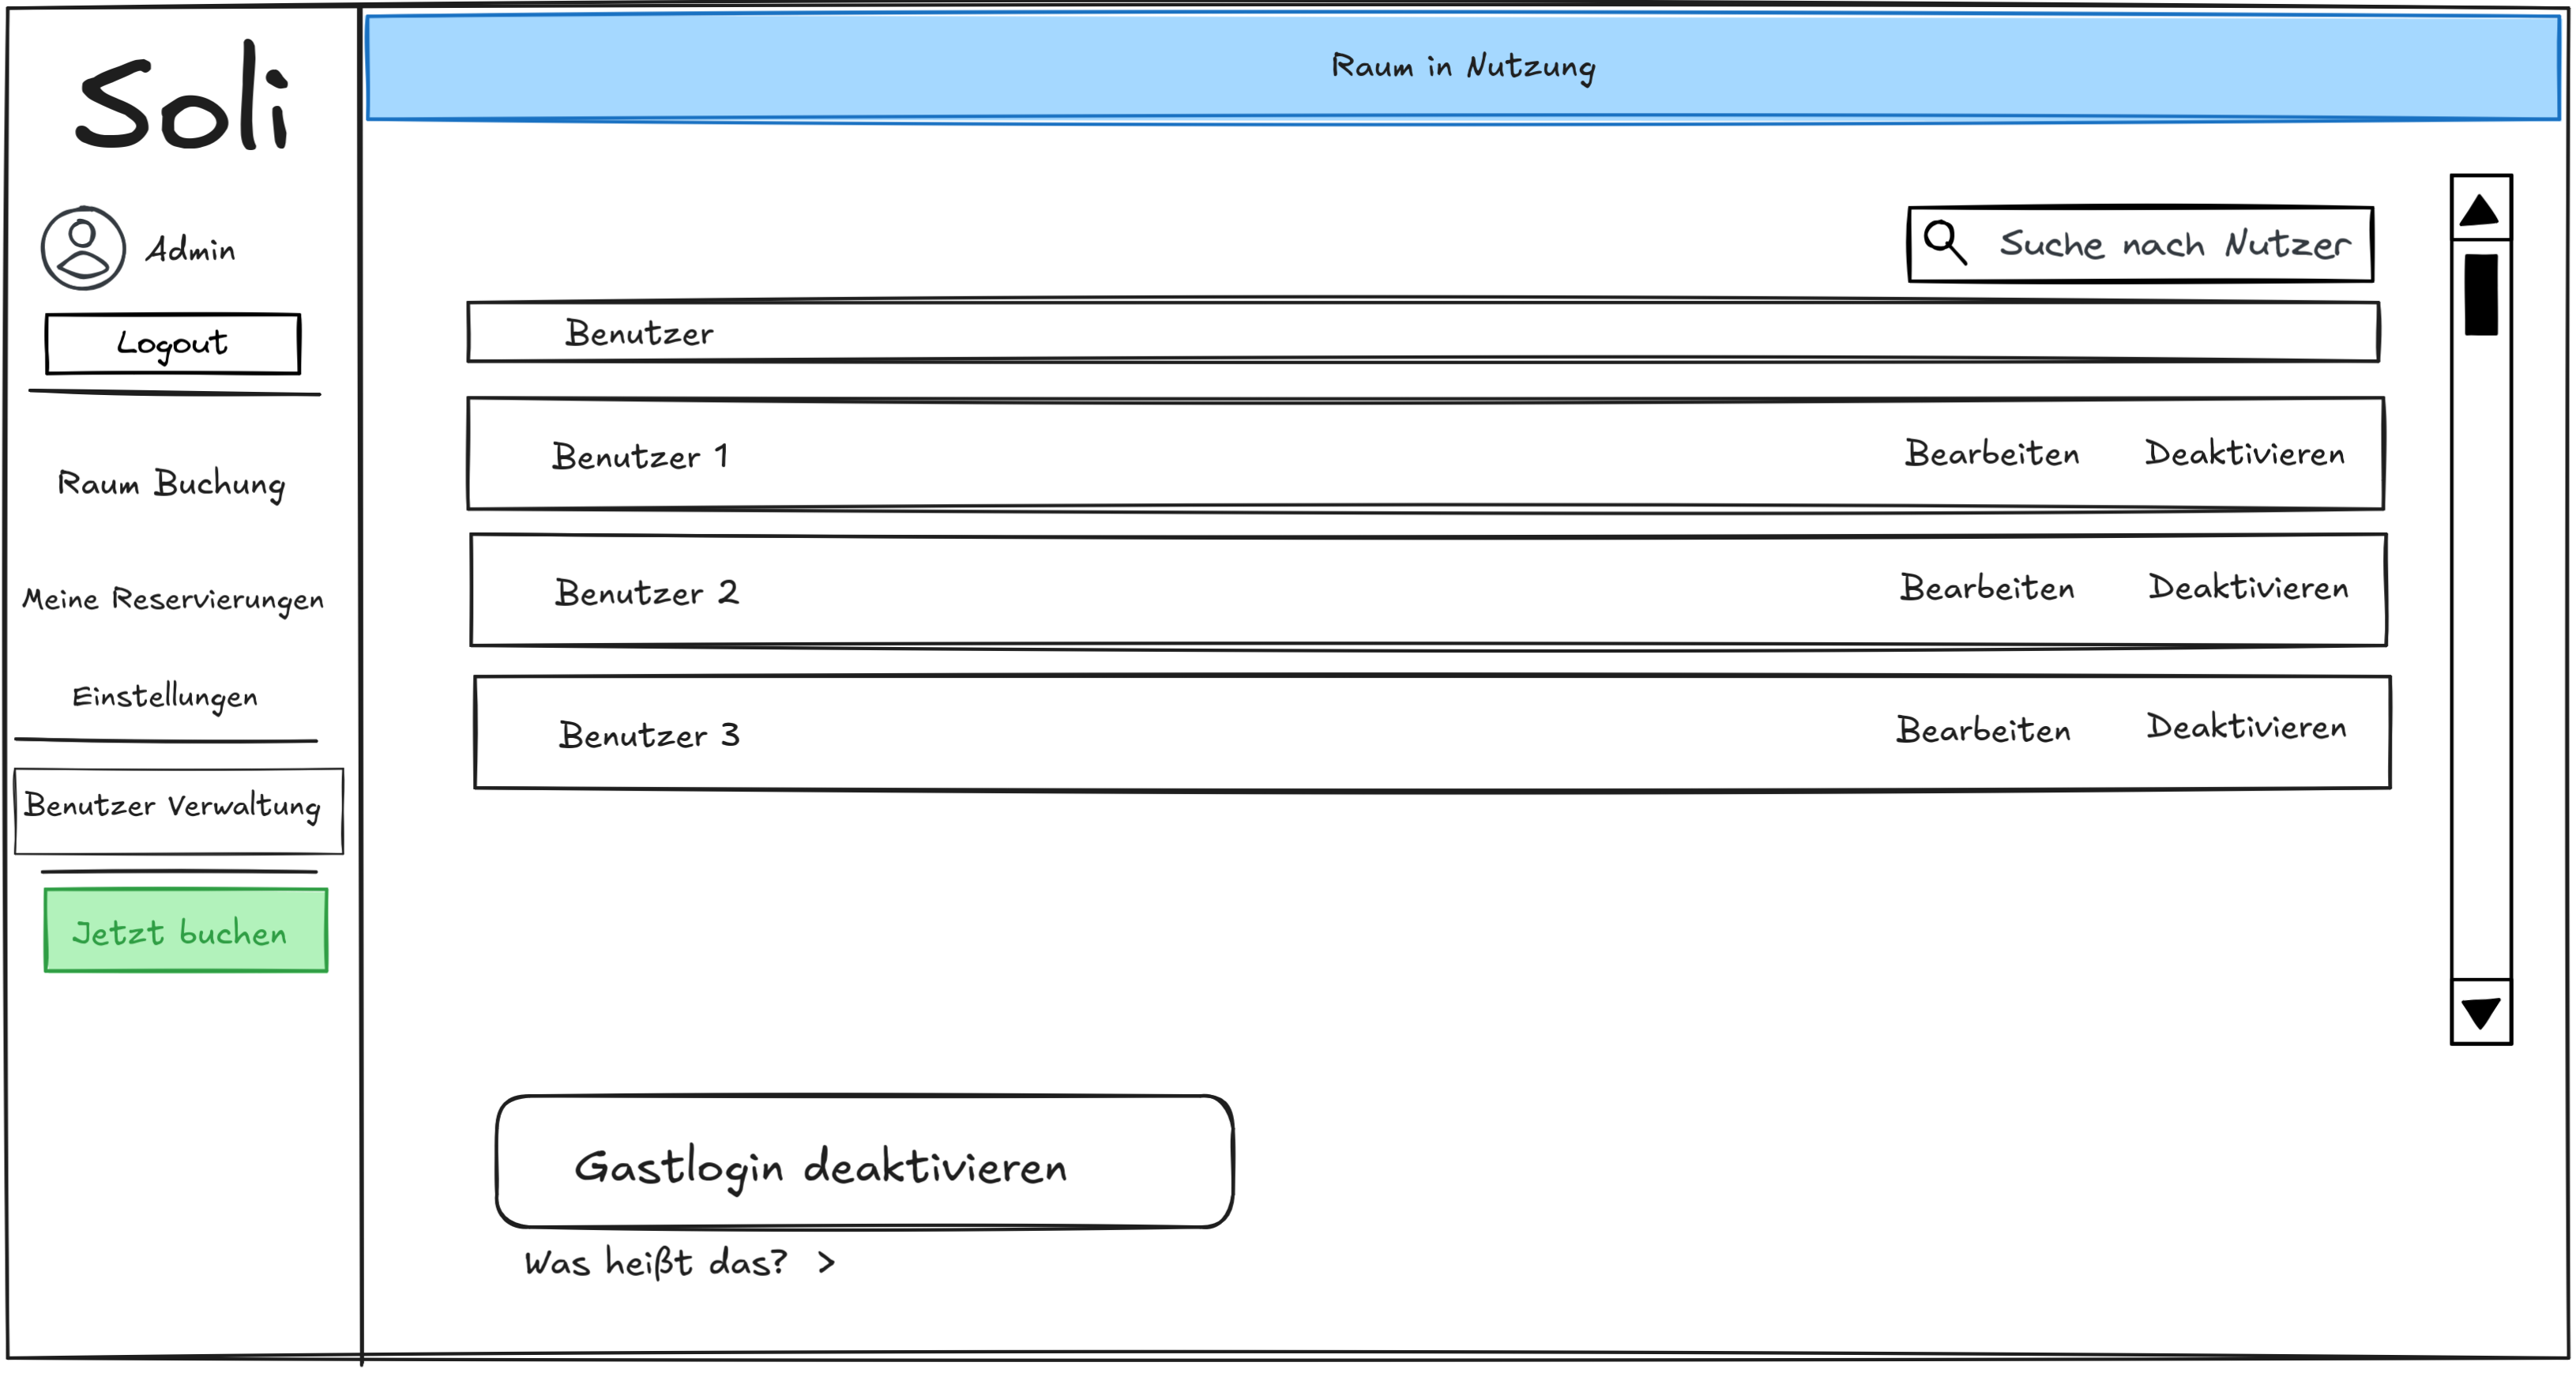
\includegraphics[width=0.65\textwidth]{pictures/figures/ui/useradminui}
        \caption{Nur für Admins zugänglich.}
        \label{fig:kontenliste}
    \end{figure}
\end{frame}

\begin{frame}[plain]
    \begin{figure}
        \centering
        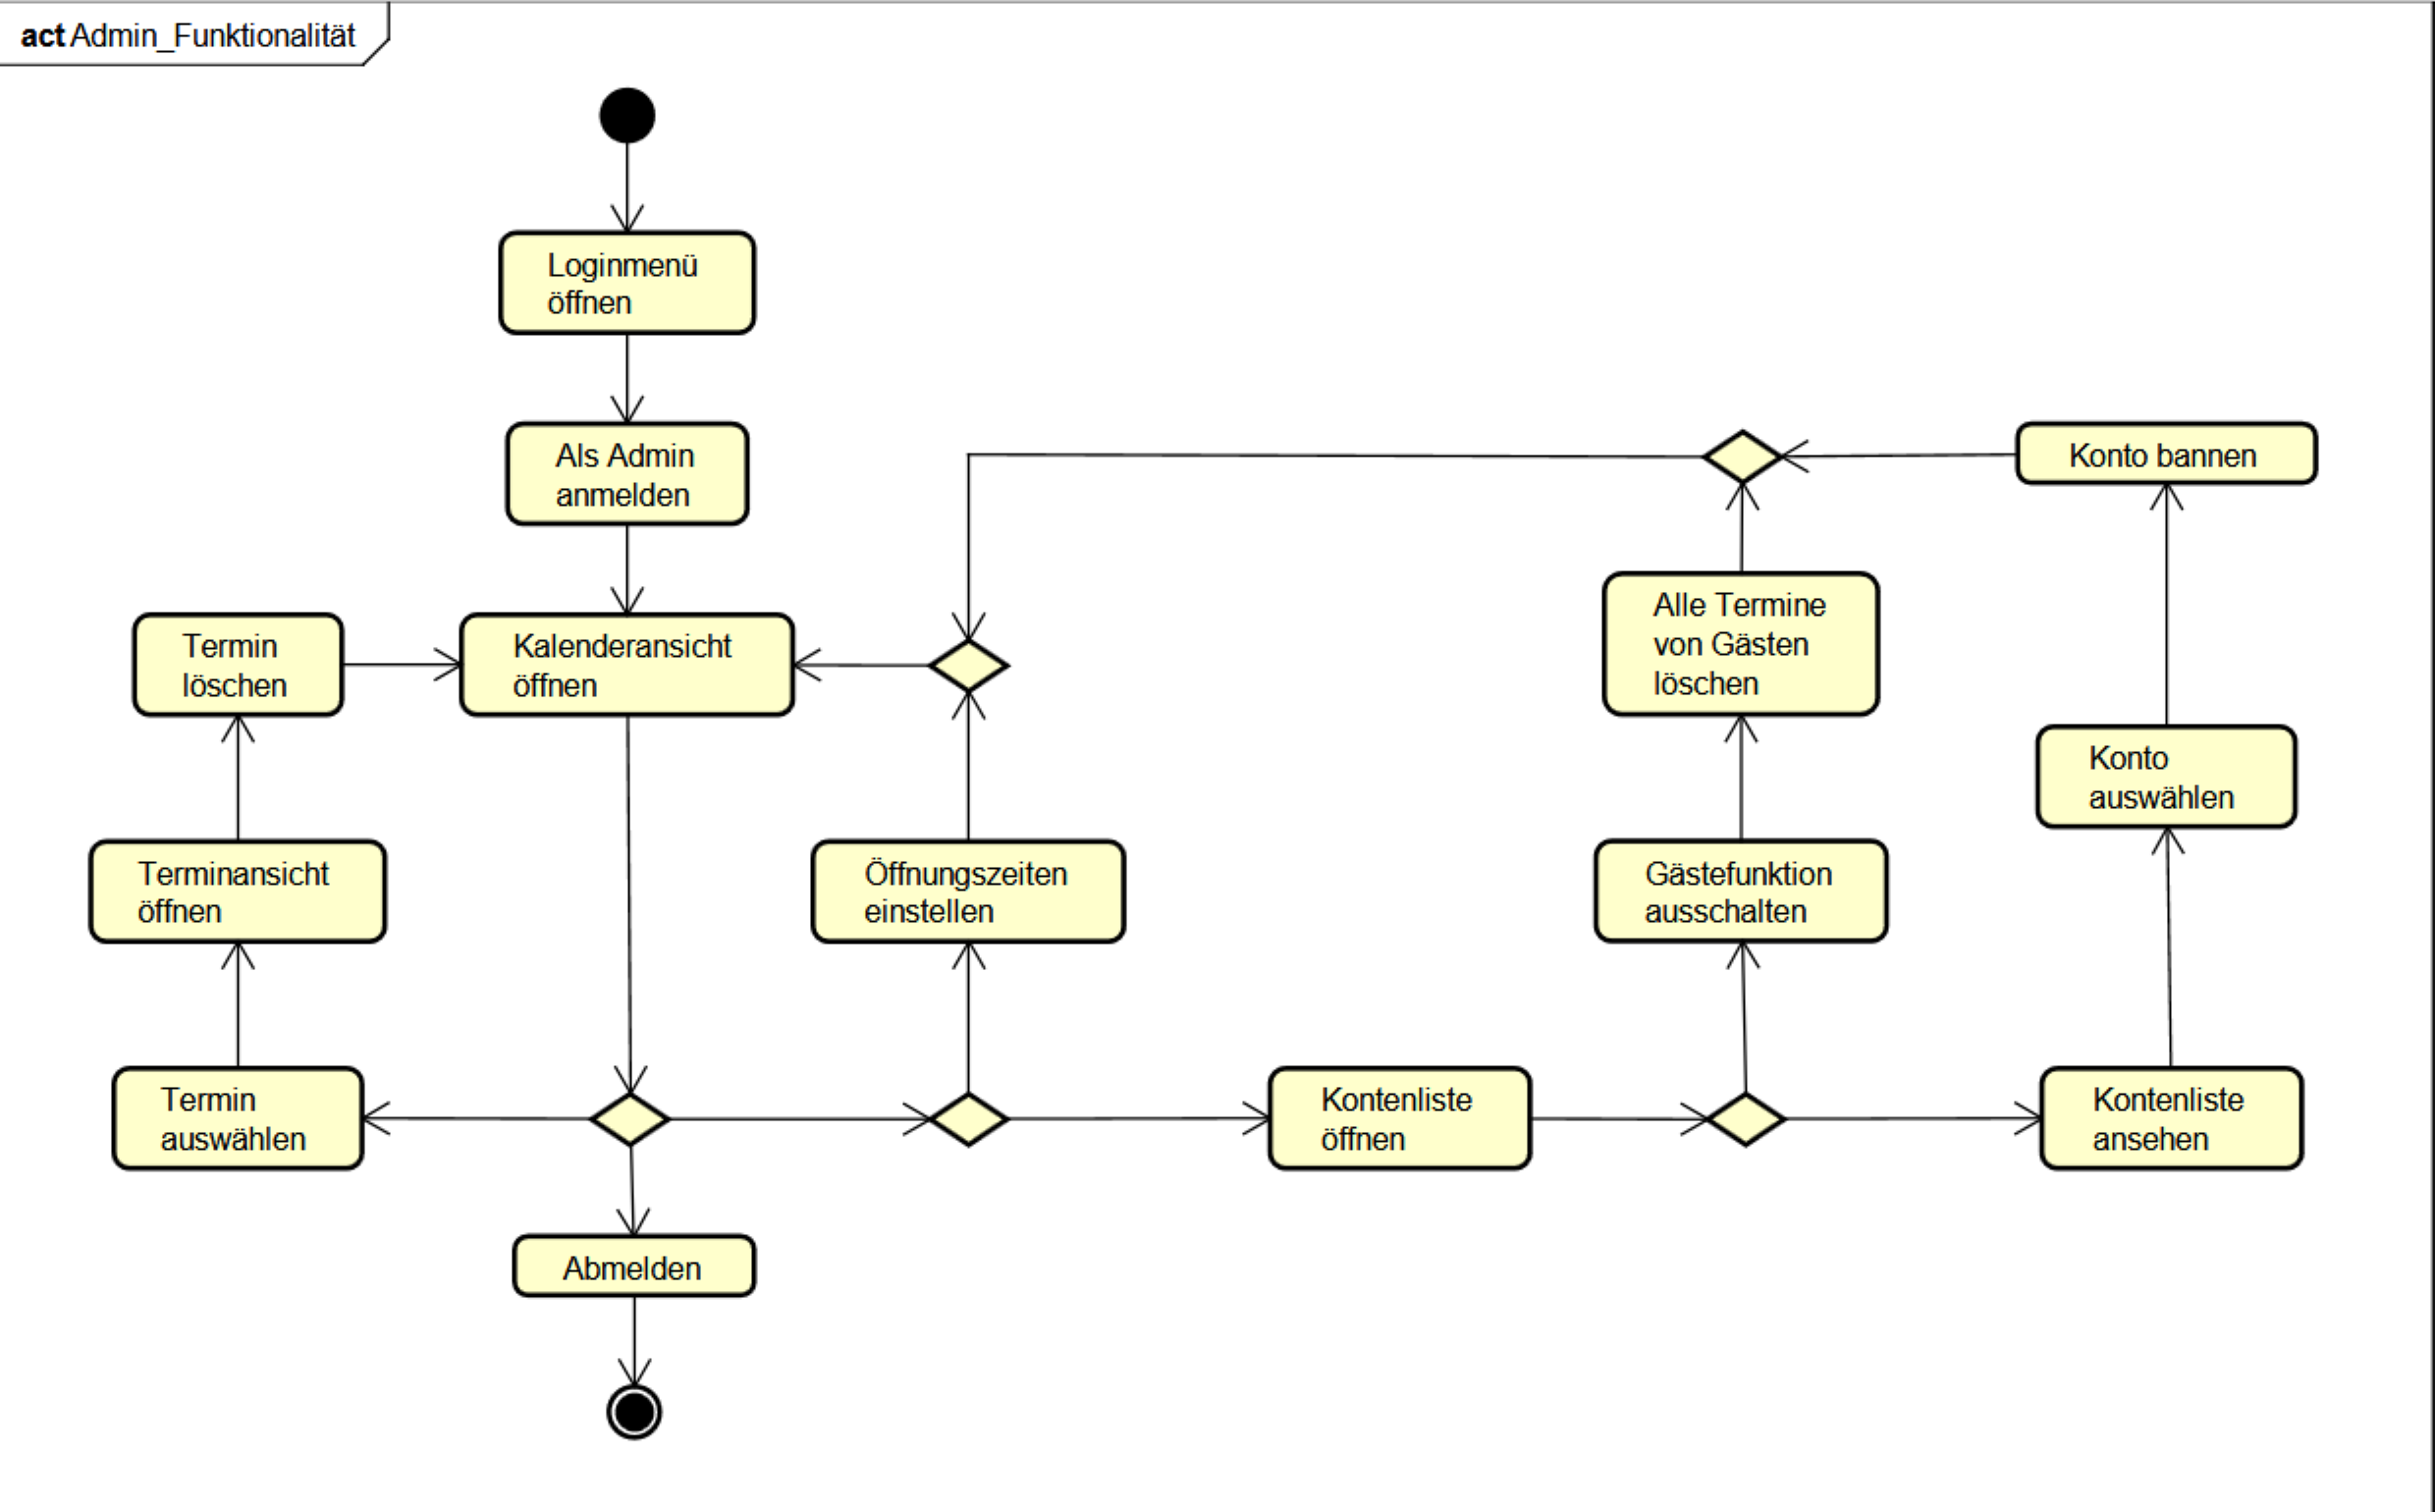
\includegraphics[width=0.95\textwidth]{pictures/figures/activity/adminfunk}
        \label{fig:adminfunktionalitaet}
    \end{figure}
\end{frame}

\section{Controller}

\begin{frame}{Controller}
    \begin{itemize}
        \item Verarbeitung von Anfragen und Erzeugung von Antworten
        \item Dekodierung und Prüfung Eingaben in HTTP-Anfragen
        \item Generierung von Parametern für JTE-Templates der View
        \item Nutzung des Service-Layers zur Datenverarbeitung
        \item Weiterleitung unangemeldeter Nutzender zur Anmeldeseite bei geschützten Endpunkten
        \item Bereitstellung von Endpunkten für die Nutzenden-Interaktion, welche die HTTP-Oberfläche kapseln und Ansichten modellieren
    \end{itemize}
\end{frame}

\subsection{Controller-Übersicht}

\begin{frame}{Controller-Übersicht (Teil 1)}
    \begin{itemize}
        \item \textbf{CalendarController:}
        \begin{itemize}
            \item Kalenderansicht und Buchungsabruf
            \item REST-Endpunkt für die Kalenderintegration mit FullCalendar
        \end{itemize}
        \item \textbf{EventFeedController:}
        \begin{itemize}
            \item REST-Endpunkt für Kalenderdaten im FullCalendar-Format
            \item Verlinkung zu den Terminansichten
        \end{itemize}
        \item \textbf{BookingViewController:}
        \begin{itemize}
            \item Terminübersicht, Terminansicht
        \end{itemize}
        \item \textbf{BookingCreateController:}
        \begin{itemize}
            \item Termin-Erstellung-Ansicht zur Verarbeitung neuer Buchungen
            \item Terminkonfliktlösung bei Überschneidungen von Buchungen
        \end{itemize}
        \item \textbf{CollaborationRequestController:}
        \begin{itemize}
            \item Formular zur Bestätigung oder Ablehnung einer Kollaboration
            \item Kollaborationsanfragen verwalten
        \end{itemize}
    \end{itemize}
\end{frame}

\begin{frame}{Controller-Übersicht (Teil 2)}
    \begin{itemize}
        \item \textbf{LoginController:}
        \begin{itemize}
            \item Login-Ansicht zur Verarbeitung der Anmeldungen (Admin, Gast, OIDC)
            \item Gastanmeldung durch E-Mail-Link
        \end{itemize}
        \item \textbf{UsersController:}
        \begin{itemize}
            \item Kontoliste für Admins
        \end{itemize}
        \item \textbf{MainController:}
        \begin{itemize}
            \item Fehlerseite anzeigen
            \item Benachrichtigungsseite bei deaktiviertem Konto
        \end{itemize}
    \end{itemize}
\end{frame}

\subsubsection{Beispiel: BookingViewController}

\begin{frame}{Beispiel: BookingViewController}
    \begin{itemize}
        \item \textbf{GET /{roomId}/bookings}
        \begin{itemize}
            \item Persönliche Terminübersicht anzeigen
        \end{itemize}
        \item \textbf{GET /{roomId}/bookings/{eventId}}
        \begin{itemize}
            \item Detailansicht eines Termins anzeigen
        \end{itemize}
        \item \textbf{DELETE /{roomId}/bookings/{eventId}}
        \begin{itemize}
            \item Termin löschen und zur Terminübersicht weiterleiten
        \end{itemize}
    \end{itemize}
    \vspace{1em}
    \textbf{Projektstruktur:}
    \begin{itemize}
        \item \textbf{RESTful Design:} Klare Trennung von Lese- und Löschoperationen
        \item \textbf{Konsistente URL-Struktur:} Einheitliches Muster für alle terminbezogenen Endpunkte
    \end{itemize}
\end{frame}

\section{Services}

\begin{frame}{Services}{Service-Layer}
    \begin{itemize}
        \item Koordination der Applikationslogik und Bereitstellung an die Endpunkte (z.B. Controller)
        \item Abkapselung der Logik der Datenverarbeitung von der Verarbeitung der HTTP-Anfragen und Antworten
        \item Verwendet Repository-Layer für die Abstraktion der Interaktion mit der Datenbank
        \item Bearbeitet komplexere Aufgaben, wie Terminbuchung, Terminkonfliktauflösung und E-Mail-Versand
    \end{itemize}
\end{frame}

\subsection{Service-Übersicht}

\begin{frame}{Service-Übersicht (Teil 1)}
    \begin{itemize}
        \item \textbf{Bookings Service:}
        \begin{itemize}
            \item Verantwortlich für Terminverwaltung (Löschen, Buchen, Koordination der Raumteilung)
            \item Bereitet Termine für die Kalenderansicht vor
            \item Identifiziert potenzielle Terminkonflikte beim Buchen und bereitet eine Auflösung vor
        \end{itemize}
        \item \textbf{E-Mail Service:}
        \begin{itemize}
            \item Ermöglicht Senden von E-Mails an die im Konto hinterlegte E-Mail-Adresse
            \item Die E-Mail-Adresse wird je nach Kontotyp vom Nutzenden oder vom OIDC-Provider bereitgestellt
        \end{itemize}
        \item \textbf{Room Service:}
        \begin{itemize}
            \item Verantwortlich für die Auswahl des Raums, der z.B. in einer Buchung verwendet wird
            \item Ermöglicht eine einfache Erweiterung der Applikation, um mehrere Räume zu verwalten
        \end{itemize}
    \end{itemize}
\end{frame}

\begin{frame}{Service-Übersicht (Teil 2)}
    \begin{itemize}
        \item \textbf{System Configuration Service:}
        \begin{itemize}
            \item Konfiguration der Applikation, z.B. der Aktivierung oder Deaktivierung von Gastkonten
            \item Wenn von einem Admin die Funktion der Gastkonten deaktiviert wird, löscht dieser Service auch alle Termine der betroffenen Konten
        \end{itemize}
        \item \textbf{User Service:}
        \begin{itemize}
            \item Verwaltet die Konten: Deaktivieren von Konten, Überprüfen des Status (Admin oder Gast), sowie das Erstellen und Löschen von Konten
        \end{itemize}
    \end{itemize}
\end{frame}

\section{Daten}

\begin{frame}{Daten}{Daten-Layer (Repository-Paket)}
    \begin{itemize}
        \item Sammlung an Schnittstellen für den Datenzugriff und die Verwaltung von Entitäten in der Datenbank
        \item Verwendet das \textbf{Spring Data JPA Framework} für die Verwaltung von CRUD-Operationen und benutzerdefinierten Abfragen
        \item \textbf{Hauptaufgaben:}
        \begin{itemize}
            \item Verwaltung von Entitäten: Es definiert Schnittstellen, die von JPA-Repository erben, um CRUD-Operationen auf den Entitäten durchzuführen
            \item Benutzerdefinierte Abfragen: Es definiert benutzerdefinierte Abfragen, um spezifische Daten aus der Datenbank zu extrahieren
        \end{itemize}
        \item \textbf{Ziel:} Trennung der Datenzugriffslogik von der Anwendungslogik
    \end{itemize}
\end{frame}

\section{Data Model}

\begin{frame}{Datenmodellübersicht}
    \begin{itemize}
        \item Das Datenmodell von Soli ist in zwei Bereiche unterteilt:
        \begin{itemize}
            \item \textbf{DTO (Data Transfer Objects):} Übertragen Daten zwischen Systemschichten
            \item \textbf{Domain:} Repräsentiert die Datenobjekte, die in der PostgreSQL-Datenbank gespeichert werden.
        \end{itemize}
        \item Das Datenmodell wird von der Datenbank in Tabellen mit definierten Beziehungen abgelegt. Daten werden nur bei aktiven Anfragen im Arbeitsspeicher gehalten und bei Bedarf in die Datenbank geschrieben.
    \end{itemize}
\end{frame}

\begin{frame}{Kernentitäten}
    \begin{itemize}
        \item \textbf{Booking:} Repräsentiert eine Buchung mit Raum, Nutzer, Zeitspanne und optionalem Kommentar
        \item \textbf{User:} Speichert die OIDC-ID der Nutzenden, ergänzt um E-Mail, Name, Sprache und den Admin-Status
        \item \textbf{Raum:} Ermöglicht die Verwaltung mehrerer Räume
    \end{itemize}
\end{frame}

\begin{frame}{Authentifizierung}
    \begin{itemize}
        \item Die Nutzenden werden über das OIDC-System des KIT identifiziert.\\ KIT-Nutzer haben IDs mit dem Präfix \texttt{kit/}, Gäste mit \texttt{guest/}, der Admin besitzt die feste ID \texttt{admin}.
    \end{itemize}
\end{frame}

\begin{frame}{Sicherheitsmaßnahmen}
    \begin{itemize}
        \item \textbf{ACID-Eigenschaften} der PostgreSQL-Datenbank gewährleisten Konsistenz und Schutz vor Datenverlust
        \item \textbf{Flyway} sorgt für automatische Datenbankmigrationen bei Modelländerungen, um Datenkonsistenz bei Systemaktualisierungen zu gewährleisten
    \end{itemize}
\end{frame}

\begin{frame}[plain]
    \begin{figure}
        \centering
        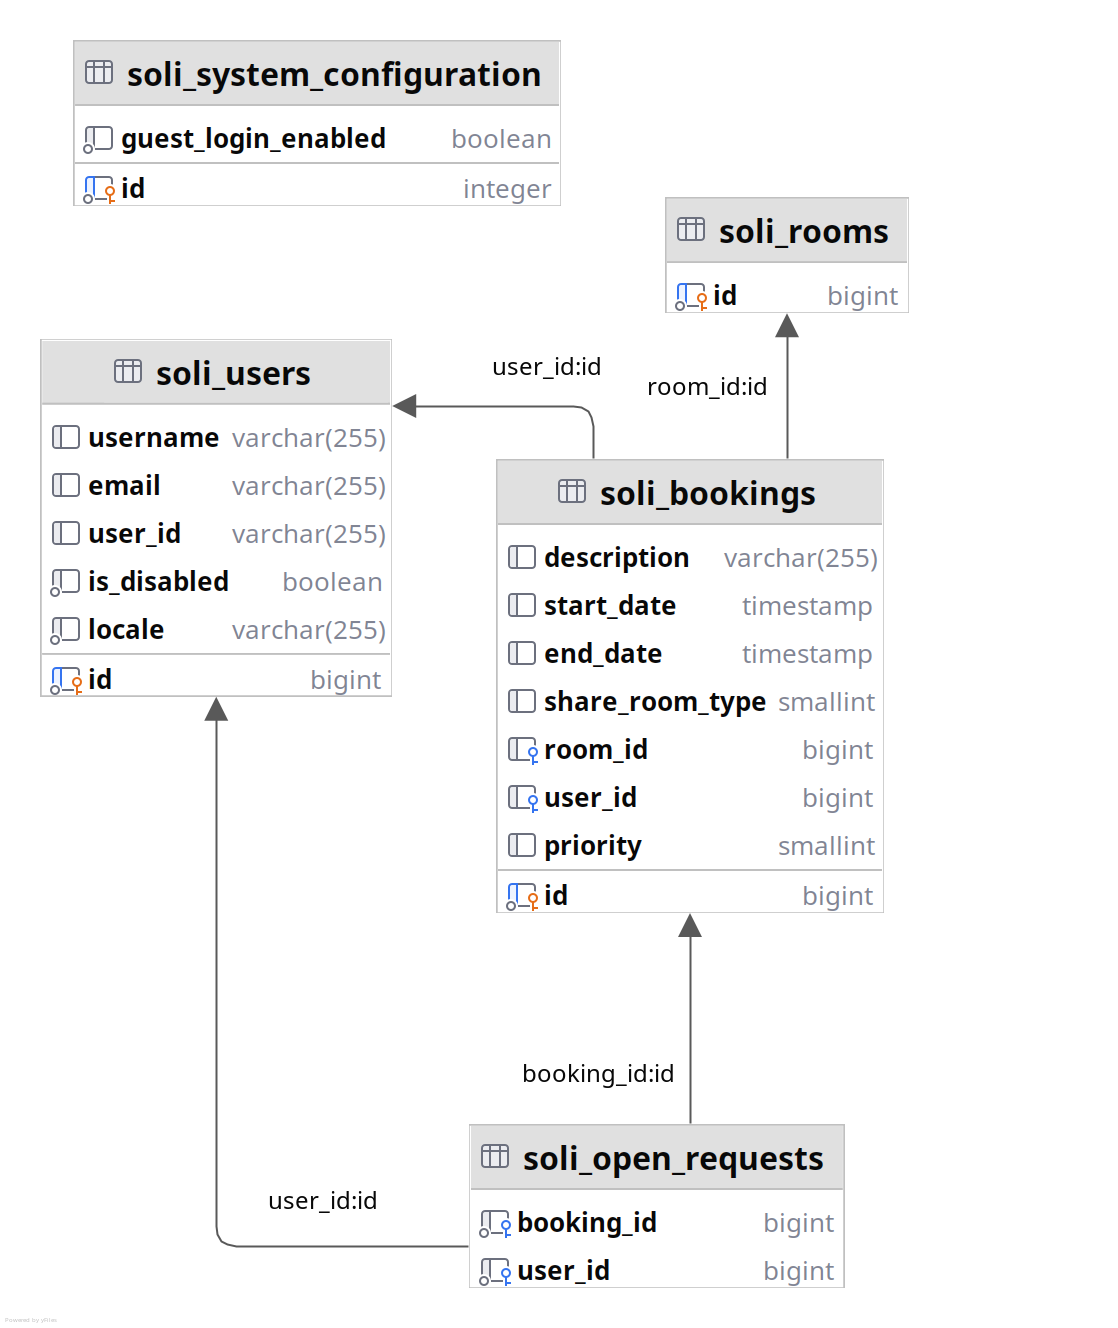
\includegraphics[width=0.45\textwidth]{pictures/figures/database}
        \caption{ER-Diagramm der Datenbank}
        \label{fig:er-diagram}
    \end{figure}

\end{frame}

\section{Q\&A}

\begin{frame}
    \centering
    \Huge \textbf{Q\&A}
\end{frame}

\end{document}